% !TEX encoding = UTF-8 Unicode

\documentclass{pclass}
\usepackage[utf8]{inputenc} % para linux y mac 
%\usepackage[latin1]{inputenc} % para windows

%DIFERENTES TIPOS DE LETRA
%\usepackage{palatino}

\usepackage{times}
\usepackage{subcaption}
\usepackage{textcomp}

\captionsetup{compatibility=false}


\begin{document}
\tipo{Grado}   % Grado o M\'aster
\titulopro{Segmentación de células en imágenes 3D con técnicas de machine learning}
\colaborador{Luis María Escudero Cuadrado\\Departamento de Biología Celular, Universidad de Sevilla}
\tutor{María José Jiménez Rodríguez}
\departamento{Matemática Aplicada I}
%\autores{Nombre 1}{Nombre 2}  % Dos autores
\autores{(ponente): Adrián López Carrillo}{{\ }}   % Un autor
\dia{27 de Septiembre de 2020 (v.1.1)}
\titulacion{Grado en Ingeniería Informática: Tecnologías Informáticas}

\hacerportada
	\makeatletter
\renewcommand*\l@section{\@dottedtocline{1}{0em}{2.5em}}
\renewcommand*\l@subsection{\@dottedtocline{2}{1.5em}{3.2em}}
\renewcommand*\l@subsubsection{\@dottedtocline{3}{4.3em}{3.2em}}
\makeatother

\renewcommand{\frontmatter}{\pagenumbering{Roman}}
%\frontmapertter

    \cdpchapter{Resumen}

En la actualidad existen microscopios que emplean técnicas ópticas para reconstruir imágenes 3D con una alta precisión. Gracias a esto los investigadores tienen a su alcance imágenes microscópicas de alta calidad para poder sacar conclusiones de ellas. Estas imágenes suelen requerir un procesado digital con el objetivo de discernir los elementos importantes del resto.

En este proyecto se abordará el problema de la segmentación de células en imágenes 3D. Para ello se usarán imágenes  cedidas por el Departamento de Biología Celular de la Facultad de Biología de la Universidad de Sevilla. En cada imágen hay decenas de células, todas en contacto con otras células sin espacio entre ellas.

El procesado digital de estas imágenes actualmente se hace de forma manual teniendo una duración de una a dos semanas, por lo que la automatización de este proceso conllevará un gran ahorro de tiempo.

Respecto a las técnicas usadas, este proyecto se centrará en el uso de redes neuronales para la segmentación de células. Se validará la efectividad del uso de redes neuronales y se estudiará qué tipo de red neuronal y arquitectura será mejor para esta tarea, teniendo en cuenta la exactitud de la segmentación y el coste computacional.

En el análisis de antecedenes se comprobará que la CNN (Convolutional Neural Network o Red Neuronal Convolucional) será con la que se obtienen mejores resultados en el reconocimiento de patrones en imágenes. También se verá que al diseñar una CNN con la arquitectura U-Net se obtienen buenos resultados.

Se probarán varios modelos de CNNs para la segmentación de células, esperándose el mejor resultado de la arquitectura U-Net.

Adicionalmente, se estudiará el uso de un preprocesado y postprocesado para aumentar la eficacia de la segmentación, así como un posterior mapeado a color de las células para ayudar a su visualización.

Esta herramienta estará disponible para el usuario final por medio de una imágen docker, para facilitar su distribución y que perdure el paso del tiempo.

%    \cdpchapter{Agradecimientos}

A nuestros alumnos y a nuestras alumnas.

	\tableofcontents % Índice de contenidos
 	\listoftables % Índice de cuadros
 	\listoffigures % Índice de figuras
% 	\lstlistoflistings %Índice de códigos

 	\mainmatter
     \part{Introducci\'on}\label{introduccion}
     \newpage
	 \thispagestyle{empty} % empty
	 \mbox{}
 	 \chapter{Nacimiento del proyecto}\label{nacimiento}

Uno de los mayores intereses del autor de este proyecto en el mundo del software siempre ha sido el uso de técnicas de inteligencia artificial para resolver problemas actuales.

Aprovechando que cursaba la asignatura de Procesamiento de Imágenes Digitales con la profesora María José Jiménez Rodríguez para preguntarle si sabía de algún TFG en el que estuviesen involucradas imágenes y pudiese desarrollar una solución de inteligencia artificial. La principal motivación par esto era que nunca había trabajado con imágenes digitales en el ámbito de machine learning.

María José habló sobre un proyecto muy interesante dirigido por el investigador Luis María Escudero Cuadrado del Departamento de Biología Celular de la Universidad de Sevilla. Parte de este este proyecto consistía en procesar imágenes 3D de glándulas salivales tomadas por un microscopio confocal para obtener la segmentación de las células. Un punto importante era que este procesado fuese automático ya que se podría ahorrar mucho tiempo, por lo que estaban valorando el uso de técnicas de machine learning.

Tras ver que este proyecto era interesante se planeó una primera visita al Departamento de Biología Celular, siendo recibidos por Luis María Escudero, Pablo Vicente-Manuera y Pedro Gómez-Gálvez. En esta reunión se habló en más detalle sobre la investigación que realizaban y el problema que se iba a abordar en el TFG.

Estaban estudiando la arquitectura a nivel celular del tejido epitelial. El tejido epitelial es uno de los 4 tejidos animales básicos, por lo que gran parte del organismo está compuesto por éste. Aunque las células de este tejido siempre se han representado en forma de prisma (cuando las células están en el mismo plano) o en forma de tronco (cuando se produce un pliegue), han demostrado que en condiciones de curvatura adoptan forma de escutoide para estabilizar energéticamente el tejido. La forma geométrica escutoide fue descubierta por este grupo de investigación \cite{GomezGalvez2018}. En la figura \ref{fig:tejidoepitelial} se pueden ver las forma de prisma, tronco y escutoide.

\figura{1}{img/tejidoepitelial}{\textbf{a} Representación de las células del tejido epitelial cuando están en una estructura plana. Se suele representar en forma de prisma. \textbf{b} Representación de las células del tejido epitelial cuando se produce un pliegue. Se suele representar en forma de tronco. \textbf{c} Geometría propuesta caracterizada por tener al menos un vértice en un plano distinto al de sus dos bases. En la figura de arriba se ven dos elementos adyacentes con forma escutoide. En la figura de abajo se ven estos elementos por separado. Las células del tejido epitelial tendrían esta geometría. (Figura editada procedente de Gómez-Gálvez et. al 2018)}{fig:tejidoepitelial}{}

Para obtener un modelo visual del tejido epitelial empiezan utilizando un microscopio confocal del que obtienen un stack de imágenes 2D, consiguiendo así una imagen 3D. Esta imagen es procesada computacionalmente utilizando herramientas de MATLAB y Fiji (ImageJ) para conseguir una imagen con todas las células etiquetadas correctamente, proceso conocido como segmentación semántica. El resultado final sería una imagen en la que cada vóxel del fondo tiene valor 0 y los vóxeles pertenecientes a cada célula tienen valor $1,2,3...n$, donde $n$ es el nº de células en la imagen. Un ejemplo de dos capas de la imagen 3D original y la imagen etiquetada puede verse en la figura \ref{fig:ejemplo1_segmentacion}

\begin{figure}[ht]
\centering
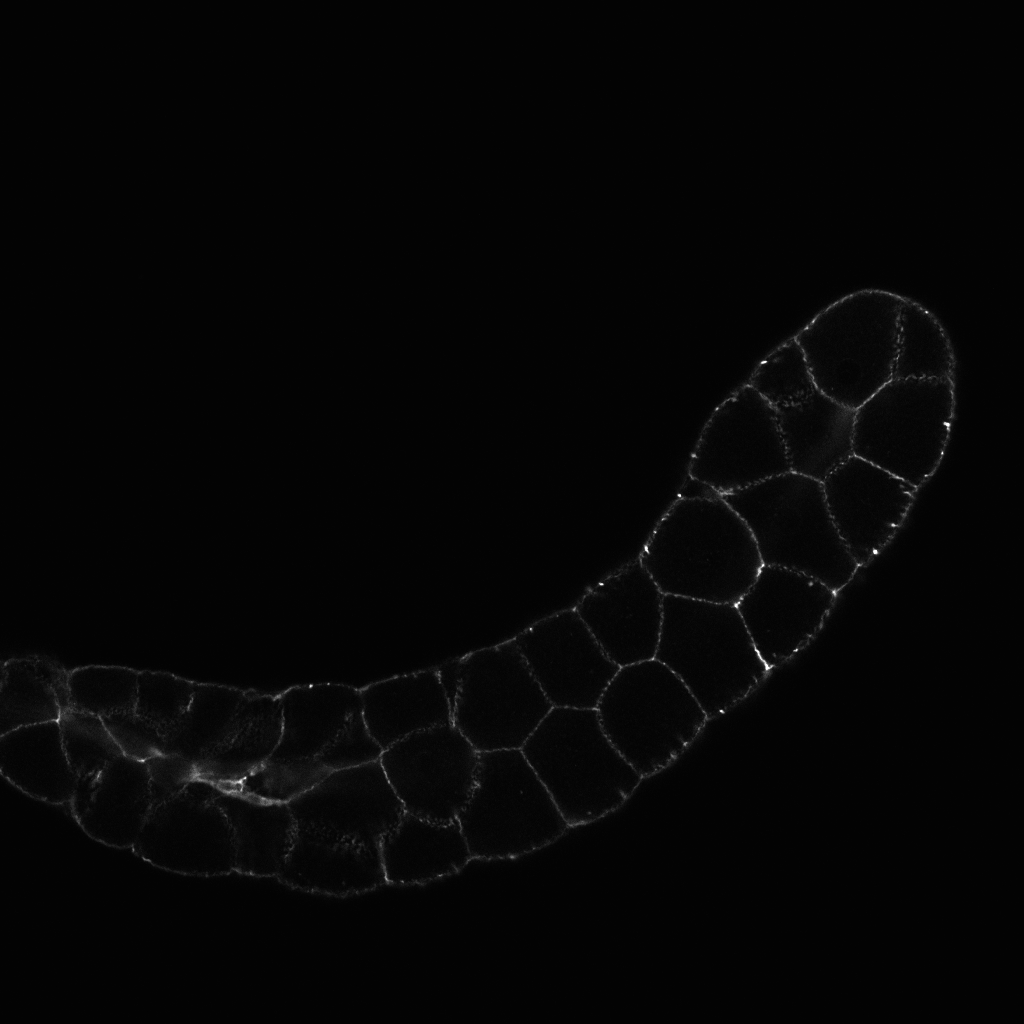
\includegraphics[scale=0.2]{img/raw 04_1a Z=77.png}
\vspace*{1mm}
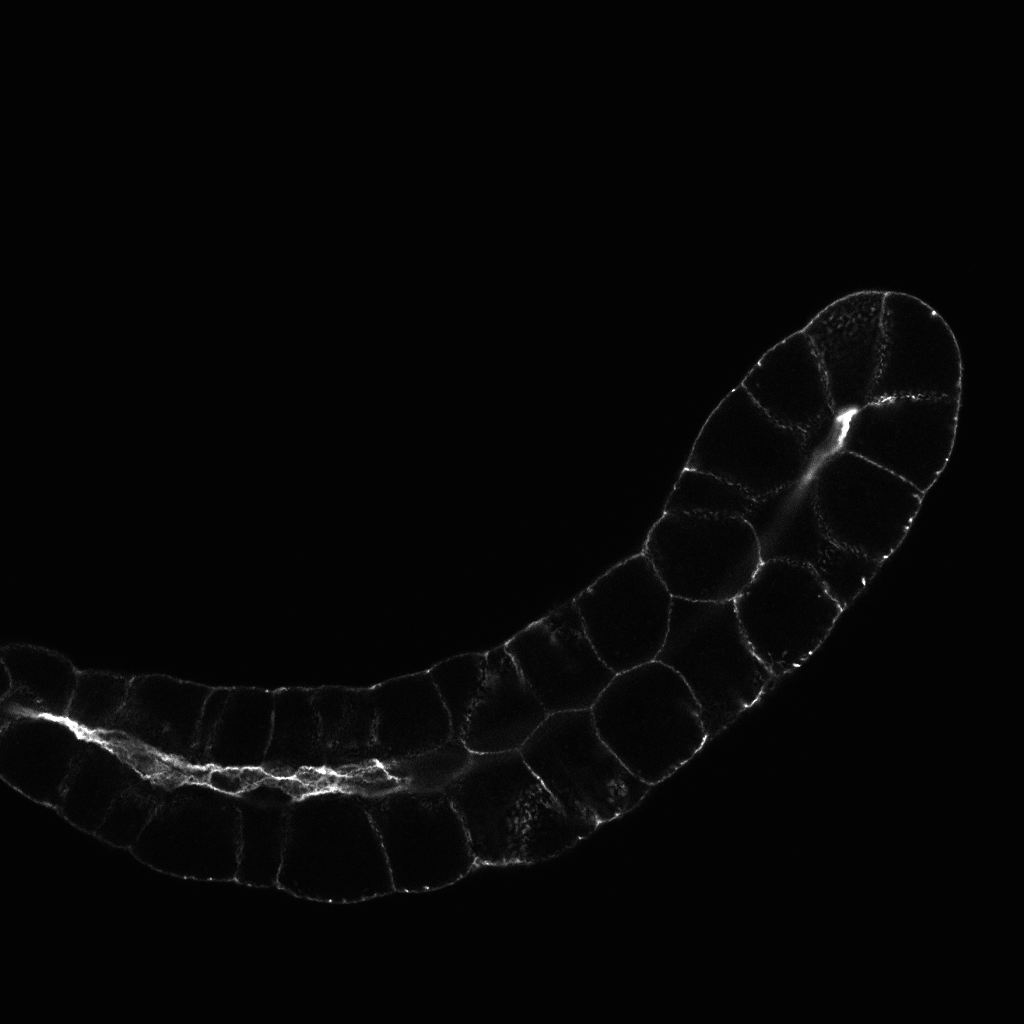
\includegraphics[scale=0.2]{img/raw 04_1a Z=100.png}
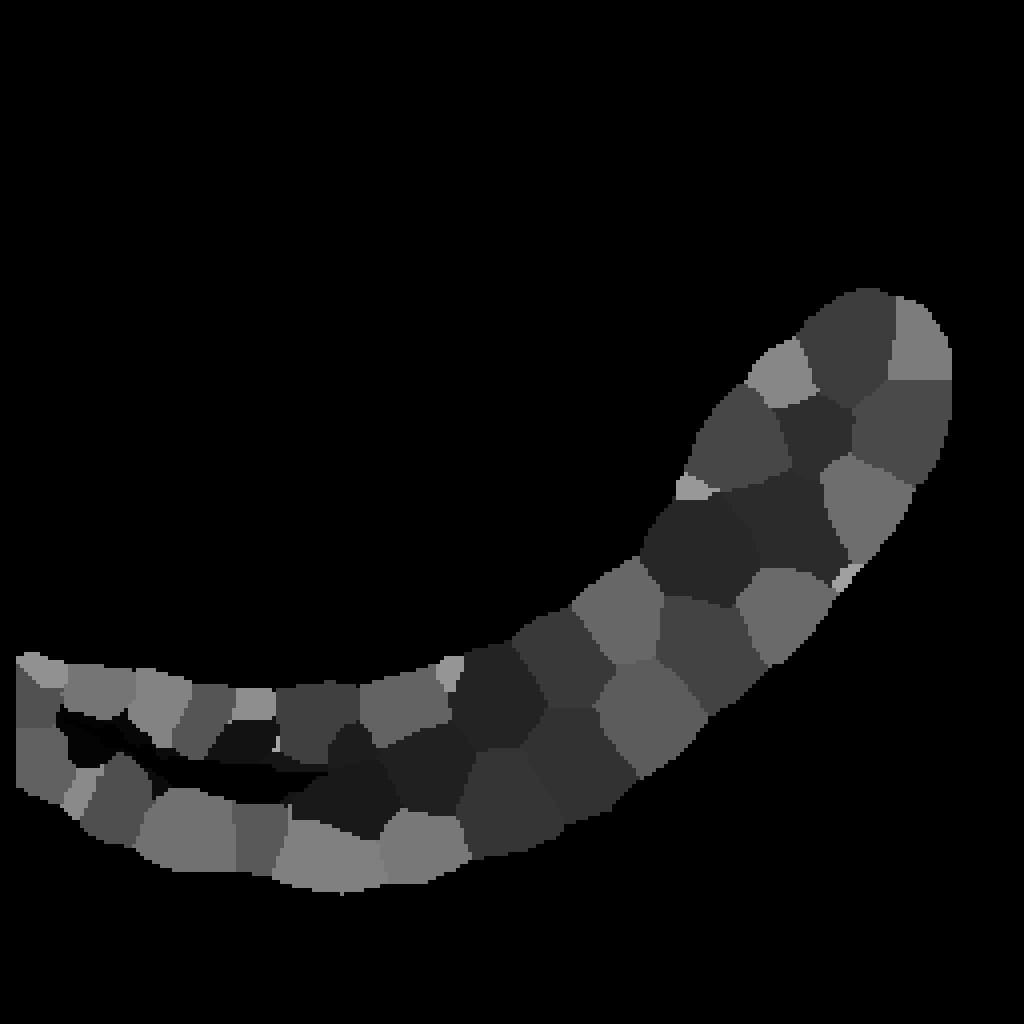
\includegraphics[scale=0.2]{img/target 04_1a Z=77.png}
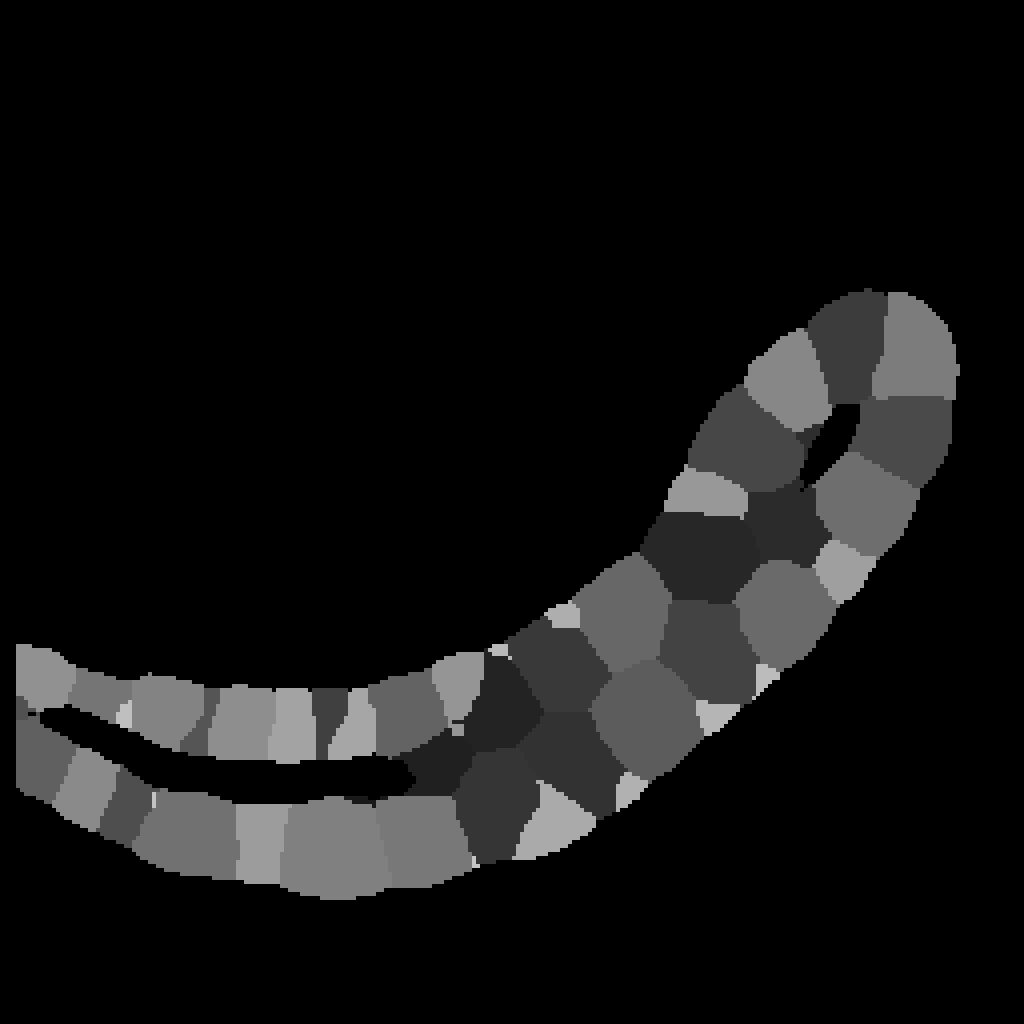
\includegraphics[scale=0.2]{img/target 04_1a Z=100.png}
\caption{Esta figura muestra el resultado de aplicar el procesado a la imagen 3D de una glándula salivar de Drosophila (un género de moscas), obtenida por microscopía. La imagen tiene las dimensiones $1024*1024*234$, seleccionándose para su representación Z=77 y Z=100. En la primera fila se muestra la imagen obtenida por microscopía y la segunda fila se muestra la obtenida al aplicar segmentación a las células. En la primera columna se muestra la capa Z=77 y en la segunda la capa Z=100.}\bigskip
\label{fig:ejemplo1_segmentacion}
\end{figure}

Pasar de la primera fila de la figura \ref{fig:ejemplo1_segmentacion} a la segunda fila es un proceso que puede llevar hasta una semana ya que se quiere conseguir un etiquetado perfecto. Esto provoca que se invierta mucho tiempo en una tarea repetitiva y poco interesante y se reste tiempo de las tareas de interés científico. Querían reducir el tiempo necesario para la segmentación y para ello pensaron que sería buena idea recurrir a técnicas de machine learning. Sería el objetivo principal del TFG, por tanto, obtener una segmentación automática que redujera el tiempo de segmentación manual, siendo lo ideal obtener directamente la segmentación perfecta.
     \chapter{Objetivos}

Este proyecto comenzó con la idea de reducir el tiempo necesario para tener una segmentación correcta de las células, por lo que ese será el objetivo principal. En las etapas iniciales del proyecto, tal y como se verá en el capítulo \ref{sec:nosetuvoencuenta} hubo un cambio de rumbo en el alcance del proyecto, es por ello que se añadió un objetivo relacionado con el coste de computación. En definitiva, los objetivos son los siguientes:

\begin{enumerate}
\item Utilizar técnicas de machine learning para desarrollar un modelo que, a partir de una imagen 3D de tejido epitelial, calcule una segmentación de las células lo más cercano posible a una segmentación perfecta.
\item Debido a que especies con distintos fenotipos pueden presentar glándulas con distinta morfología a nivel celular, es útil la posibilidad de poder entrenar un modelo con distintos datasets.
\item Debido a las dificultades encontradas en el primer acercamiento al problema, hacer que el proyecto funcione correctamente con una capacidad de computación limitada.
\item Debido a que el proyecto será utilizado por personal del ámbito científico y no tecnológico, hacer que el proyecto sea de uso e instalación sencilla.
\end{enumerate}
	 \part{Organizaci\'on del Proyecto}\label{organizacion}
	 \newpage
	 \thispagestyle{empty} % empty
	 \mbox{}	 
	 \chapter{Planteamiento inicial}\label{planinicial}

\section{Plan inicial}\label{sec:planinicial}

El primer enfoque para abordar este proyecto fue utilizar herramientas actuales de machine learning para la segmentación semántica de las imágenes provistas y, a partir de los resultados obtenidos, investigar cómo mejorar la segmentación. Sin embargo esto no fue posible debido a la alta resolución de las imágenes provistas y al limitado acceso a hardware de alto rendimiento. Por ello se ideó un plan inicial en el que se construía una herramienta que tuviese menor requisito de hardware. La mayor limitación era por la VRAM necesaria, por lo que se pensó en utilizar Apache Spark \cite{apachespark} para aprovechar HDD y RAM.

En este primer plan se dividieron las tareas en fases, siendo la fase 0 realmente un proceso de iniciación, necesaria para planificar el resto de las fases.

\begin{itemize}
\item[\textbf{Fase 0}] Estudio previo. Investigar las soluciones actuales al problema o problemas similares, las posibles técnicas de machine learning a usar en este proyecto y tecnologías para implementarlas.
\item[\textbf{Fase 1}] Aprender a implementar una CNN en Python. Usar datos de prueba para familiarizarme con las tecnologías a usar en este proyecto. Se explica en más detalle por qué usar CNN en la sección \ref{sec:archs}. El uso de Python se explica en la sección \ref{subsec:language}.
\item[\textbf{Fase 2}] Implementar, entrenar y probar una o más CNN.
\item[\textbf{Fase 3}] Analizar resultados obtenidos.
\item[\textbf{Fase 4}] Investigar sobre mejoras pre y post procesado.
\item[\textbf{Fase 5}] Realizar estas operaciones usando Apache Spark. Framework que facilita trabajar con datos a gran escala aprovechando HDD y RAM.
\item[\textbf{Fase 6}] Hacer que el entrenamiento y la inferencia sean usables por un usuario.
\end{itemize}

\section{Nueva metodología}\label{sec:metodologia}

Gracias a la investigación inicial realizada en la \textbf{Fase 0} se pudo definir el resto de fases del plan inicial, aunque no se tuvieron en cuenta varios factores que se empezaron a ver en la \textbf{Fase 1} y \textbf{Fase 2}. Esto provocó que se tuviese que realizar un ajuste en el plan inicial. 
Lo que no se tuvo en cuenta fue:

\begin{itemize}
\item Las fases 2, 3 y 4 deben ser fases iterativas. Cada vez que se obtengan resultados hay que estudiarlos y hacer cambios para mejorar los resultados.
\item No se tiene en cuenta el rendimiento de los algoritmos utilizados ni los cuellos de botella.
\item Se quiere usar Spark con la premisa de aprovechar la RAM o el HDD cuando la VRAM se agote, pero esto no es viable ya en la VRAM se tiene que poder almacenar toda la información necesaria para ejecutar cada algoritmo.
\end{itemize}

Por todo ello, se buscó información sobre una metodología adecuada. El capítulo 11 del libro Deep Learning \cite{Goodfellow2016} habla sobre una metodología práctica para la aplicación de técnicas en deep learning. Esta metodología se centra en utilizar feedback del sistema construido en cada iteración para modificar el sistema acorde a los objetivos. Los pasos a seguir propuestos por esta metodología son:

\begin{enumerate}
\item Determinar las metas. Qué métrica usar como error y un valor de la métrica aceptable como objetivo.
\item Establecer lo antes posible un sistema completo que pueda dar un valor para dicha métrica.
\item Utilizar herramientas adecuadas para determinar cuellos de botella en el rendimiento. Comprobar qué componentes están dando peores resultados en el sistema y comprobar si los resultados negativos son debidos a overfitting, underfitting, a un fallo con los datos o en el software.
\item Hacer cambios de forma a los datos, ajuste de hiperparámetros o cambiar algoritmos con el objetivo de mejorar la métrica usada. Volver al punto 3.
\end{enumerate}

Estos pasos se resumirán como ``desarrollo del sistema" y constituirá la mayor parte del proyecto.
\newpage
\section{Plan seguido}\label{sec:planactualizado}

\begin{itemize}
\item[\textbf{Fase 0}] Estudio previo. En esta fase se investigará sobre artículos de segmentación celular y se aprenderá sobre machine learning y las tecnologías necesarias para llevar a cabo resultados similares aplicados al problema actual.
\item[\textbf{Fase 1}] Desarrollo del sistema. Aplicar la metodología de la sección \ref{sec:metodologia}.
\begin{enumerate}
\item Determinar metas con métricas.
\item Sistema inicial.
\item Usar herramientas para determinar cuellos de botella en el rendimiento.
\item Cambios en el sistema.
\item Si no se ha alcanzado el valor objetivo de la métrica, volver al punto 3.
\end{enumerate}
\item[\textbf{Fase 2}] Mejoras de usabilidad. Que el proyecto sea usable por un usuario.
\item[\textbf{Fase 3}] Cierre. Terminar de escribir la memoria con los resultados obtenidos, las conclusiones, tabla de tiempos y manual de usuario.
\end{itemize}

	 \chapter{Costes}\label{costes}


	 \part{Estudio previo}\label{estudioprevio}
	 \newpage
	 \thispagestyle{empty} % empty
	 \mbox{}
	 \chapter{Red Neuronal Artificial}\label{redneuronal}

En este capítulo se hará un recorrido histórico haciendo énfasis en los avances del siglo XX en redes neuronales artificiales (ANNs). Después se definirá la neurona artificial y se distinguirán 3 tipos: perceptrón, sigmoide y unidad lineal rectificada (ReLU). Estos serán los tipos de neurona artificial más frecuentes en los algoritmos usados en este proyecto. Por último se hablará sobre el entrenamiento de la ANN.

\section{Introducción a Redes Neuronales Artificiales}\label{subsec:nn_intro}

Desde la antigüedad la humanidad ha sentido interés en la posibilidad de emular la inteligencia de forma artificial. Con los avances en neurociencia hemos sido capaces de entender cómo funcionan las neuronas, la unidad básica en el funcionamiento de los cerebros. Siendo el cerebro un ejemplo funcional de un sistema inteligente, es natural  que haya interés en replicar su funcionamiento.\\

Un hito importante se produjo gracias al desarrollo de la teoría del aprendizaje biológico, introducida por Warren McCulloch y Walter Pitts en 1943 \cite{McCulloch1943}, popularizando lo que fue llamado como \emph{cibernética} \cite[p13]{Goodfellow2016}. Gracias a esto surgió el ADALINE (elemento lineal adaptativo) \cite{Widrow2015}, que es un caso concreto del algoritmo descenso por gradiente estocástico (\textbf{SGD}), algoritmo que con pequeñas modificaciones es usado en la actualidad en el proceso de aprendizaje\cite[p14]{Goodfellow2016}. Fue también gracias al estudio de McCulloch y Pitts que en 1958 Frank Rosenblatt introdujo por primera vez el \textbf{perceptrón}, un modelo general de neurona artificial \cite{Rosenblatt1958}, que fue perfeccionado por Minsky Y Papert en 1969 \cite{Minsky1969}.

El perceptrón es un modelo lineal que, dado un conjunto de elementos con dos categorías distintas como entrada, puede clasificar cada elemento en una de esas dos categorías. Un ejemplo sencillo son las puertas lógicas, siendo la entrada un conjunto de dos elementos con las categorías 0 o 1 y la salida sería un 0 o un 1.

Minsky y Papert encontraron un problema en los modelos lineales y lo demostraron con la función XOR, siendo imposible para un modelo lineal compuesto de una neurona artificial aprender esta función. Esto causó un declive en el interés sobre este campo.\\

En la década de 1980 resurgió el interés gracias en parte al conexionismo, cuya idea central es que un gran número de unidades de computación simples pueden tener un comportamiento inteligente al estar conectadas entre sí \cite[p16]{Goodfellow2016}. Durante esta etapa se hicieron importantes contribuciones como la representación distribuida \cite{Hinton1986}, donde se habla sobre representar las entradas de un sistema en base a sus características, reconocidas por patrones de actividad en redes neuronales. Otra gran contribución fue la populariación del algoritmo de propagación hacia atrás, \textbf{ backpropagation} \cite{Rumelhart1986} para entrenar redes neuronales artificales y actualizar sus pesos, siendo este algoritmo el más usado en la actualidad. 

En este punto de la historia los algoritmos más importantes involucrados en las redes neuronales artificiales usadas en la actualidad habían sido descubiertos, pero no se estaban obteniendo resultados tan buenos como los esperados. Desde un principio lo que se había estado buscando era replicar de forma artificial el funcionamiento del cerebro, siendo el cerebro un sistema de computación genérico, capaz de aprender todo tipo de conocimiento distinto sin la necesidad de cambiar su arquitectura o su método para aprender. Era imposible conocer el algoritmo de aprendizaje usado en el cerebro ya que para ello haría falta monitorizar una gran cantidad de neuronas con gran precisión, lo cual es imposible incluso en la actualidad.\\

En 2006 se produjo un hito importante que comenzó la etapa del \textbf{aprendizaje profundo}, cuando Geoffrey Hinton demostró que era posible entrenar de forma eficiente una red neuronal profunda con un gran número de capas ocultas \cite{Hinton2006}.

\section{Neurona artifical}\label{subsec:neurona_artificial}

En la figura \ref{fig:generic_computing_unit} se puede ver una neurona artifical genérica con la que pueden ser descritos los distintos tipos que se verán en esta sección.

\figura{1}{img/Rojas1996_p31_computing_unit}{Neurona artificial genérica}{fig:generic_computing_unit}{}

Siendo:
\begin{itemize}
\item $ (x_1, x_2, ...,x_n) $ el vector de entrada.
\item $ (w_1, w_2, ...,w_n) $ el vector de pesos.
\item $ g $ la función de integración, encargada de reducir el vector de entrada a un único valor.
\item $ f $ la función de activación, encargada de producir la salida de este elemento.
\end{itemize}

Se puede simplificar la representación al asumir que siempre se usará $ \sum x_i w_i $ como función de integración. Además toda neurona artificial tendrá una entrada y un peso por defecto, independientemente del vector de entrada, esto hará referencia al \textit{bias}. Será común ver una representación como \ref{fig:neurona_artificial} en la que $ f $ indicará la función de activación.

\figura{1}{img/NeuronaArtificial}{Representación de una Neurona Artificial con $ \sum x_i w_i $ como función de integración}{fig:neurona_artificial}{}

\begin{itemize}
\item Al vector de entradas se le añade un elemento de valor constante 1, siendo ahora de tamaño $ n+1 $.
\item Al vector de pesos se le añade un elemento de valor inicial $ -\theta $, siendo ahora de tamaño $ n+1 $. A este valor se le llamará \textit{bias}.
\item $ f $ indicará la función de activación de la neurona artificial.
\end{itemize}

\subsection{Sigmoide}\label{subsubsec:sigmoide}

La función sigmoide como función de activación es una función no lineal usada principalmente en redes neuronales prealimentadas (feedforward neurals networks), que son las que usaremos en este proyecto. Es una función real, acotada y diferenciable (a diferencia de la usada en el perceptrón). Su definición es la siguiente relación \cite{nwankpa2018activation}:

\begin{equation}
 f(x) = \sigma (x) = \frac{1}{1+e^{-x}}
\end{equation}

\subsection{Unidad Lineal Rectificada (ReLU)}\label{subsubsec:relu}

La unidad lineal rectificada (ReLU) fue propuesta como función de activación en 2010 por Nair y Hinton \cite{Nair2010} y desde entonces ha sido la más usada en aplicaciones de aprendizaje profundo (deep learning, DL). Si se compara con la función de activación Sigmoide, ofrece un mejor rendimiento y es más generalista \cite{nwankpa2018activation}.

\begin{equation}
 f(x) = max(0, x)=\left\{\begin{matrix}
 x_i & $si $ x_i \geq 0 \\ 
 0 & $si $ x_i < 0
\end{matrix}\right.
\end{equation}

\newpage\section{Red Neuronal Artifical}\label{subsec:neural_network}

Considerando la neurona artificial como una unidad de computación básica, según el conexionismo (que más tarde evolucionó en lo que hoy conocemos como \textit{deep learning}, se podría emular un comportamiento inteligente al conectar neuronas artificiales entre sí. La conexión entre las neuronas artificales se consigue concatenando las salidas de unas con la entradas de otras y obteniendo así una red neuronal artifical (ANN).

\figura{1}{img/neural_network}{Red Neuronal Artificial completamente conectada.}{fig:neurona_artificial}{}

En la figura \ref{fig:neurona_artificial} se ve una Red Neuronal Artifical completamente conectada (\textit{fully connected neural network} o FCNN) en la que todos los nodos de una capa están conectados con todos los nodos de la capa siguiente. Contaría con los siguientes elementos:
\begin{itemize}
\item Capa de entrada $i$ (\textit{Input layer}) con $ n $ nodos. Cada nodo representa un valor del vector de entrada $ x $. En esta capa no se altera el valor de $x$, está para representar los pesos de cada elemento del vector de entrada con los nodos de la primera capa oculta.
\item Capas ocultas $(h1, h_2, ..., h_m)$ (\textit{hidden layers}). Cada capa oculta podrá tener un nº de nodos distintos. Es en estas capas donde se reconocen los patrones del conjunto de datos y tiene el mayor coste computacional. La última capa oculta está conectada con las entradas de la capa de salida.
\item Capa de salida $o$ (\textit{output layer}) con $c$ nodos. La última capa de la red neuronal, la salida de esta capa nos dará un vector de tamaño $c$ como salida.
\end{itemize}

\section{Descenso por Gradiente }\label{sec:gradient_descent}

En cálculo de varias variables calcular el gradiente de una función ($\nabla f$) dará como resultado un vector indicando la dirección en la que esa función tiene un mayor incremento, siendo el módulo el ritmo de variación. Para el descenso del gradiente será interesante usar $-\nabla f$ ya que nos dará el vector en el que la función decrece más. Como es habitual en problemas de optimización, si suponemos que tenemos una función que nos da el error cometido, nuestro objetivo será minimizar dicha función.

La función a optimizar se llamará \textbf{función de pérdida} (\textit{loss function}) en la que se comparará la salida obtenida por la red con la salida deseada. Hay que tener que este es un algoritmo de aprendizaje y sólo tendrá sentido usarlo cuando se conozca el resultado correcto para una entrada determinada.

La salida obtenida por una red para una entrada determinada y, por lo tanto, el valor obtenido en la función de pérdida, dependerá únicamente de los pesos de dicha red. Esto significa que lo ideal será encontrar el mínimo global de la función de pérdida al cambiar el valor de los pesos de la red. Para actualizar los pesos se usará la fórmula $w_{ij} = w_{ij} - \eta \nabla J(W)$ donde $w_ij$ es el peso desde el nodo $i$ al nodo $j$, $\eta$ es el factor de aprendizaje o \textbf{learning rate} y $\nabla J(W)$ es la función de coste dados unos pesos determinados.

No es extraño en deep learning encontrar una red con millones de pesos pero, para facilitar la visualización, se ha usado como ejemplo una ANN con 2 pesos ($\theta_0$ y $\theta_1$). En la figura \ref{fig:gradient_descent} se puede ver una ilustración de cómo en cada punto (marcado por una X negra) se calcula el gradiente de $J(\theta_0, \theta_1)$ y se actualizan los pesos, cambiando el valor de $J(\theta_0, \theta_1)$ hasta alcanzar un mínimo.

\figura{1}{img/gradient_descent}{Ilustración del algoritmo de descenso por gradiente. $\theta_0$ y $\theta_1$ son los pesos de la ANN y $J$ la función de pérdida. Se puede observar cómo se produce un "descenso" hacia un mínimo de la función.}{fig:gradient_descent}{}

	 \chapter{Red Neuronal Convolucional}\label{cnn}

En este capítulo se estudiarán los fundamentos de la red neuronal convolucional (CNN), un subtipo de ANN especializado en el tratamiento de imágenes y usado por aplicaciones actuales de segmentación semántica \ref{apps}.\\

Hasta ahora se ha supuesto que la entrada a una ANN es un vector, algo válido para un gran número de aplicaciones en deep learning. El problema está cuando la entrada de la red neuronal es una imagen. En este caso antes de utilizar la imagen como entrada hay que aplanarla para contener la imagen en un vector, de esta forma cada píxel (o vóxel) será un elemento del vector de entrada y estará conectado a cada neurona de la capa siguiente. Para el caso de imágenes pequeñas (como la de la figura \ref{fig:image_to_ANN}) puede ser viable, pero teniendo tan sólo una imagen de $4$x$4px$ y 4 neuronas en la única capa oculta, se tendrían $16*4=64$ pesos. Si aplicáramos este sistema a una imagen 3D en escala de grises con $124*124*70=1076320vx$, se necesitarían más de un millón de pesos por cada neurona que haya en la primera capa oculta. Esto hace que sea completamente inviable usar este tipo de redes para imágenes a partir de cierto tamaño. En este capítulo se presentan las redes neuronales convolucionales (CNN), que reducirán en gran medida el nº de pesos necesarios en la red neuronal y aprovecharán técnicas del procesamiento de imágenes para encontrar patrones.

\figura{0.8}{img/image_to_ANN}{Imagen de 4x4 px aplanada y usada como entrada en una FCNN con 4 neuronas en su única capa oculta. No se muestra su capa de salida. Imagen del curso Intro to Deep Learning with PyTorch de Udacity.}{fig:image_to_ANN}{}{Imagen como entrada en una ANN.}

Cambiando la arquitectura de la red vista en la figura \ref{fig:image_to_ANN} por una CNN, obtendríamos una arquitectura similar a la vista en la figura \ref{fig:image_to_CNN}. En esta CNN se ha reducido el nº de conexiones de la capa de entrada a la capa oculta de $64$ a $16$, además, como veremos más adelante, los pesos de las 4 neuronas son compartidos, esto significará que sólo se necesitarán $4$ pesos distintos.

\figura{1}{img/image_to_CNN_}{Imagen de 4x4 px usada como entrada en una CNN. Ambas figuras muestran la misma arquitectura, estando en la figura de la izquierda la imagen aplanada y en la figura de la derecha se muestra la matriz 4x4 como entrada. Imágenes del curso Intro to Deep Learning with PyTorch de Udacity.}{fig:image_to_CNN}{}{Imagen como entrada en una CNN.}

\subsubsection{Conceptos de procesamiento de imagen}

Antes de describir los tipos de capas será necesario introducir varios conceptos propios del procesamiento de imagen que son usados en la capa convolucional (subsección\ref{cnn_capa_conv}) y la capa pooling (subsección \ref{cnn_capa_pooling})

Lo primero es saber que una convolución es una operación matemática entre dos funciones ($f$ y $g$) que produce una tercera función ($f*g$) que expresa cómo la forma de $f$ es cambiada por $g$. \cite{wikipedia_convolution}

En este caso $f$ será la imagen original y $g$ será una matriz con el mismo número de dimensiones que la imagen. Para facilitar esta explicación se asumirá que la imagen original tiene dos dimensiones, aunque en este proyecto se trabaje con imágenes de tres dimensiones.

Siguiendo este esquema, a $g$ se le conocerá como \textbf{kernel} y definirá la naturaleza de la operación realizada a lo largo de $f$. Si se tiene un kernel $X$ de tamaño $(m,m)$ y una imagen $Y$, esta operación respecto al punto $(y_1, y_2)$ de $Y$ puede definirse cómo la ecuación \ref{eq:kernel}, con un ejemplo visual en la figura \ref{fig:kernel}:

\begin{equation}\label{eq:kernel}
\sum_{k=0}^{m-1}\sum_{l=0}^{m-1} X_{j,k} * Y_{y_1 - i-\lfloor l/2 \rfloor, y_2 -  j -\lfloor l/2 \rfloor}
\end{equation}

\figura{0.4}{img/kernel}{Kernel $2$x$2$ aplicado al elemento $(0,0)$ de una matriz $3$x$3$. Imagen tomada de  d2l.ai.}{fig:kernel}{}{Resultado de aplicar un kernel a una imagen.}

En la figura \ref{fig:kernel} se puede observar un problema al intentar aplicar el kernel al punto $(0,2)$. El kernel ``se sale" de la imagen, por lo que no se puede computar esta operación y se pierde información. Para solucionar esto se aplica lo que se conoce como \textbf{padding}.

El padding es una técnica que consiste en añadir píxeles de relleno alrededor de una imagen. En este contexto se añade 0 para evitar alterar los resultados. Un ejemplo de de padding puede verse en la figura \ref{fig:padding}

\figura{0.5}{img/padding}{Kernel $2$x$2$ aplicado al elemento $(0,0)$ de una matriz $3$x$3$ con padding 1 aplicado. Imagen tomada de  d2l.ai.}{fig:padding}{}{Resultado de aplicar un kernel a una imagen con padding.}

Esta operación se debe realizar para toda la imagen de entrada. Si se quiere realizar esta operación para todos los puntos de la imagen, el kernel debe ``deslizarse" sobre la imagen elemento a elemento, tanto en horizontal como en vertical. En este caso se dirá que se tiene un \textbf{paso} de 1 horizontal y vertical. En la imagen \ref{fig:paso} se puede ver un ejemplo con un paso horizontal de 2 y vertical de 3. De aquí en adelante se supondrá que el paso horizontal y vertical tienen el mismo valor, por lo que el paso estará definido por un solo número.

\figura{0.5}{img/paso}{Kernel $2$x$2$ aplicado a una matriz $3$x$3$ con padding 1, paso horizontal 2 y vertical 3. Imagen tomada de d2l.ai.}{fig:paso}{}{Resultado de aplicar un kernel a una imagen con padding y pasos 2 y 3 para horizontal y vertical.}

Al determinar el kernel, paso y padding se definirá un \textbf{filtro}. Los filtros son de gran interés en el procesamiento de imagen ya que al aplicarlos se pueden producir efectos como enfoque, realce o detección de bordes. En la figura \ref{fig:filtro} \ref{WikipediaFiltro2020} se muestra un ejemplo de aplicar un filtro a una imagen de entrada.

\begin{figure}[ht]
\centering
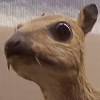
\includegraphics[scale=2]{img/filter_og.png}
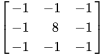
\includegraphics[scale=1]{img/filter_edge_kernel.png}
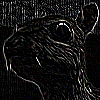
\includegraphics[scale=2]{img/filter_edge.png}
\caption[Resultado de aplicar un filtro de reconocimiento de bordes a una imagen.]{Efecto producido al aplicar un filtro de detección de bordes a una imagen de entrada. Imágenes tomadas de la página ``Núcleo (procesamiento digital de imágenes)"\phantom{x} de Wikipedia.}\bigskip
\label{fig:filtro}
\end{figure}

\section{Tipos de capas}\label{cnn_capas}

Antes de describir los tipos de capa usados para construir una  CNN es importante mencionar la \textbf{profundidad}. Cada capa tendrá una profundidad asociada que no hay que confundir con la profundidad de una ANN. En una CNN si una capa tiene profundidad $k$, querrá decir que en esa capa hay un stack de $k$ imágenes en escala de grises. Lo normal es que cada imagen del stack represente características distintas de la imagen de entrada.

A continuación se describirán las capas más comunes usadas en una CNN: Capa Convolucional, Capa de Pooling, Capa ReLU y Capa Completamente Conectada (FC). En la figura \ref{fig:simple-convnet} \cite{missinglink2020} se puede ver un ejemplo en el que la imagen de un barco pasa por varias capas de convolución + ReLU, Pooling y por último FC, dando la predicción de la clase de la imagen.

\figura{1}{img/simple-convnet}{Red Neuronal Convolucional simple en la que la imagen de un barco es clasificada.}{fig:simple-convnet}{}{Ejemplo de CNN en la que se clasifica una imagen con un barco.}

\subsection{Capa convolucional}\label{cnn_capa_conv}

Es la capa principal de este tipo de redes, es donde se aplican los filtros a las imágenes usando convoluciones. Es descrita por 4 hiperparámetros:

\begin{itemize}
\item Número de filtros, \textbf{K}.
\item Tamaño del kernel, \textbf{F}.
\item Paso, \textbf{S}.
\item Padding, \textbf{P}.
\end{itemize}

Esta capa va a tener como entrada una imagen con una profundidad $K_0$, le aplicará un padding de \textbf{P} píxeles/vóxeles alrededor de la imagen y realiza la operación de convolución del stack de imágenes y de $K$ filtros de tamaño $F$ en todas sus dimensiones excepto en la dimensión de la profundidad, que será de tamaño $K_0$. El paso con el que desplazamos los filtros sobre las imágenes será $S$. Suponiendo que la imagen inicial tiene 2D, esta operación se hará frente a una entrada de tamaño $W_1 \times H_1 \times D_1$ y dará como resultado una imagen de tamaño:

\begin{itemize}
\item $W_2 = \frac{W_1 - F}{S} + 1$
\item $H_2 = \frac{H_1 - F}{S} + 1$
\item $D_2 = K$
\end{itemize}

De la misma forma que se han calculado $W$ y $H$ se puede calcular cualquier nº de dimensiones. También es importante notar que aunque se puede elegir cualquier valor para $S$, $F$ y $P$, es habitual en las arquitectura modernas que las convoluciones se realicen con $S=1$, $F=3$ y $P=1$, de esta forma quedaría: $W_2 = \frac{W_1-F+2P}{S} + 1 = \frac{W_1 - 3 + 2}{1} + 1 = W_1$. Haciendo esto no varía el tamaño de la imagen.

En la figura \ref{fig:conv-example}\cite{Li2020} se muestra un ejemplo de una capa de convolución de profundidad $2$ con imagen de entrada $5 \times 5$ con $1 px$ de padding y profundidad $3$, siendo los filtros de tamaño $3$ y aplicándose con un paso de $3$. Se obtendrá una imagen $3\times 3$ con profundidad $2$.

Para que la salida tenga profundidad $2$ será necesario usar $2$ filtros. Cada uno de estos filtros tendrá un kernel de tamaño $3\times 3 \times n$, siendo $n=3$ la profundidad de la imagen de entrada a esta capa. Cada kernel tendrá 27 valores, uno por cada píxel. Estos valores son los pesos de las neuronas de la red neuronal y no están definidos por el usuario como los hiperparámetros, en cambio se incializarán de forma aleatoria y se irán modificando acorde al algoritmo de optimización utilizado. Entrenar una CNN significa encontrar unos valores para los filtros que minimicen el error (dado por la función de pérdida). Adicionalmente, también habrá que entrenar la capa FC, que no es más que una red neuronal como ya se ha visto previamente.

\figura{0.8}{img/conv-example}{Capa de convolución de profundidad 2 (se usan dos filtros) con kernel de tamaño $3\times 3 \times 3$ aplicado a una imagen de entrada de tamaño $5\times5$ con profundidad 3 y padding 1. El resultado es un volumen de $3x3x2$.}{fig:conv-example}{}{Ejemplo de capa de convolución.}

\newpage\subsection{Capa Pooling}\label{cnn_capa_pooling}

El objetivo de esta capa es reducir el tamaño de las imágenes para reducir la memoria necesaria y el coste computacional.

De forma similar a la capa de convolución, en la capa de pooling o reducción se usa un filtro que se aplica a toda la imagen. Se diferencian en que esta capa usa un solo filtro de profundidad $1$ que es aplicado a todas las imágenes del stack de entrada, por lo que esta capa mantiene la misma profundidad de la capa anterior. Otra diferencia está en la operación a realizar, en la capa de convolución se aplica un kernel con determinados valores a toda la imagen, en la capa de pooling se la función MAX.

Los parámetros necesarios para definir una capa de pooling son:
\begin{itemize}
\item Tamaño del kernel, $F$.
\item Paso, $S$.
\end{itemize} 

Y si se tiene una entrada de tamaño $W_1 \times H_1 \times D_1$, la salida será:
\begin{itemize}
\item $W_2 = \frac{W_1 - F}{S} + 1$
\item $H_2 = \frac{H_1 - F}{S} + 1$
\item $D_2 = D_1$
\end{itemize}

Los parámetros $F$ y $S$ determinan cómo se reducirá la imagen, siendo común usar $F=2$ y $S=2$ para reducir el tamaño a la mitad. Reducir demasiado la imagen al hacer pooling puede provocar un efecto muy destructivo.

\figura{1}{img/maxpool}{Imagen $4\times 4$ a la que se ha aplicado un pooling de $F=2, S=2$. Cada color de la imagen de la izquierda indica las entradas del para la operación MAX, cada color de la imagen de la derecha indica la salida de dicha operación. Figura tomada del curso ``CS231n" de Standford University.}{fig:maxpool}{}{Ejemplo de pooling.}

\subsection{Capa ReLU}\label{cnn_capa_relu}

Esta capa aplica la función de activación no lineal \textit{ReLU} (vista en el apartado \ref{subsubsec:relu}) a cada elemento (píxel o vóxel) de la entrada. Se introduce después de la capa de convolución y es a veces llamada la etapa de detección \cite[335]{Goodfellow2016}.

\subsection{Capa FC}\label{cnn_capa_fc}

Se usa para obtener la puntuación de clase de cada píxel/vóxel de la capa anterior, a la que está completamente conectada (cada nodo de la capa anterior está conectado a todos los de esta capa). Es la salida de la red ya que es la última capa. En problemas de clasificación esta capa tendrá $C$ nodos, siendo $C$ el nº de clases. En problemas de segmentación esta capa tendrá tantos nodos como clases haya multiplicado por el nº píxeles/vóxeles que haya en la capa anterior, entendiéndose la segmentación como etiquetar cada píxel/vóxel con la probabilidad que tiene de pertenecer a cada clase.

Esta capa funciona como una ANN normal, incluyendo los pesos y su actualización.

\section{Funciones de Pérdida}\label{cnn_loss_func}

En esta sección se describirán varias funciones de pérdida que se tuvieron en cuenta en el capítulo \ref{loss_function}, seleccionando finalmente la entropía cruzada binaria.

En las CNNs, al igual que en la inmensa mayoría de algoritmos de Deep Learning, se usa el descenso por gradiente estocástico o alguna variación como método para optimizar y aprender hacia un objetivo. En este proyecto el objetivo viene dado por la segmentación perfecta realizada de forma manual a la que se llamará $y$. Esta segmentación perfecta se comparará con la predicción obtenida ($\hat{y}$) por el modelo CNN al tomar como dato de entrada la imagen original sin procesar. Como se vio en la sección del descenso por gradiente (\ref{sec:gradient_descent}), se usará una función que tome como entrada la segmentación perfecta y la predicción y devuelva un valor numérico indicando cuánto se aleja la predicción del objetivo. Esta función será la función de pérdida. A continuación se describirán varias funciones de pérdida en relación con el problema de segmentación semántica.

\subsection{Binary Cross-Entropy}\label{cnn_bce}

La entropía cruzada binaria es una medida utilizada para calcular la diferencia entre dos distribuciones de probabilidad. \cite{Jadon2020}. Resultará útil si comparamos el objetivo $y$ con la predicción $\hat{y}$. La fórmula de la entropía cruzada binaria (BCE) es la siguiente:
\begin{equation}
L_{BCE}(y,\hat{y})=-(y log(\hat{y}) + (1-y)log(1-\hat{y}))
\end{equation}

\subsection{Weighted Binary Cross-Entropy}\label{cnn_wbce}

La entropía cruzada binaria con pesos (WCE) es una variante de BCE. En esta variante se aplica un coeficiente a cada ejemplo positivo. Es muy útil cuando los datos están sesgados, como por ejemplo una segmentación de un elemento muy pequeño en comparación con el fondo. La formula es la siguiente:
\begin{equation}
L_{WBCE}(y,\hat{y})=-(\beta y log(\hat{y}) + (1-y)log(1-\hat{y}))
\end{equation}

Para reducir el número de falsos negativos usar $\beta > 1$, para reducir el número de falsos positivos usar $\beta < 1$ \cite{Jadon2020}.

\subsection{Dice Loss}\label{cnn_dice}

El coeficiente Dice se usa como métrica para calcular la similitud entre dos imágenes. En 2016 se adaptó para usarlo como función de pérdida \cite{Cardoso2017}. La fórmula es la siguiente:
\begin{equation}
DL(y,\hat{p})= 1 - \frac{2y\hat{p}+1}{y+\hat{p}+1}
\end{equation}

Siendo $\hat{p}\epsilon[0,1]$ la probabilidad de que un píxel/vóxel pertenezca a una clase, dada por la predicción del modelo, siendo la suma de todas todas las probabilidades (para un determinado píxel/vóxel) igual a $1$.

Se le añade $1$ en el numerador y denominador para evitar que haya $0$ en el numerador o denominador.


	 \chapter{Arquitecturas para segmentación semántica}\label{sec:archs}

En este capítulo se verán varias arquitecturas que popularizaron técnicas importantes en deep learning y redes convolucionales en concreto. El objetivo será llegar a la arquitectura U-Net, ya que será la utilizada durante este proyecto, que será implementada en el capítulo \ref{full_unet}.

En los últimos años se han desarrollado diversas arquitecturas para CNN consolidándola como el mejor método actual para resolver ciertos problemas en tratamiento de imágenes, como la clasificación o la segmentación. Esto ha sido posible gracias en parte a los avances obtenidos en el reto ImageNet \cite{Deng2009}. 
ImageNet es una base de datos con más de 10 millones de imágenes etiquetadas a mano, entre las que hay 1000 categorías distintas. Desde 2010 se ha organizado una compteción anual donde los participantes tienen que desarrollar y entrenar el mejor modelo para clasificar estas imágenes. 
\begin{itemize}
\item El ganador del reto de 2012 fue un equipo de la Universidad de Toronto con la arquitectura AlexNet \cite{Krizhevsky2012}, usando filtros 11x11 y siendo el primer modelo en usar ReLU como función de activación, algo que se ha convertido en estándar.
\item En 2014 VGGNet (VGG), del Grupo de Geometría Visual de la Universidad de Oxford, fue de los que obtuvo mejor resultado en la competición con 2 versiones distintas, VGG16 con 16 capas y VGG19 con 19 capas \cite{Simonyan2014}. Ambas versiones emparejan convolución y pooling, usan filtros para las capas de convolución, 2x2 para las capas de pooling, acabando la red en 3 capas completamente conectadas. VGG fue el primer modelo en usar filtros tan pequeños, mostrando que se obtenían mejores resultados al hacerlo.
\item El ganador del reto de 2015 fue ResNet, desarrollada por Microsoft Research \cite{He2015}. ResNet utiliza una misma distribución de capas repetida durante toda la red. Posee 152 capas, siendo la primera vez que se alcanzaba un número tan alto de capas de forma práctica. Era difícil tener tantas capas a causa del problema del desvanecimiento de gradiente \cite{Hochreiter1998} que se da al entrenar por backpropagation y resulta en que, al hacer la propagación hacia atrás, cada capa consecutiva reduce el error propagado llegando ``desvanecerse'', resultando en un difícil entrenamiento. Esto es solucionado por ResNet al conectar capas lejanas para que el error pueda propagarse entre estas más rápido, llamando a estas conexiones \textit{skip connections}.
\end{itemize}

Estas arquitecturas resultaron en hitos importantes para el desarrollo de CNN, a continuación se describirán varias arquitecturas para segmentación semántica.

\newpage\section{Fully Convolutional Network}\label{sec:fcn}

Fue propuesta en 2014 por investigadores de la Universidad de California en Berkeley \cite{Long2014} obteniendo los mejores resultados hasta la fecha en segmentación semántica mediante el uso de redes convolucionales. Un punto clave fue tomar una entrada de un tamaño arbitrario y producir una salida de un tamaño correspondiente. Usa como base los modelos AlexNet, VGGNet y GoogLeNet \cite{Szegedy2014}, donde se sustituyeron las capas completamente conectadas con capas convolucionales con filtros 1x1 y añadieron una capa convolucional con filtro 1x1 y profundidad C+1 para predecir las puntuaciones de cada clase, C el nº de clases y añadiendo una más para el fondo.

Se compararon los modelos FCN-AlexNet, FCN-VGG16 y FCN-GoogLeNet, obteniendo los mejores resultados con FCN-VGG16 y convirtiéndose este en el modelo base. Con el objetivo de ganar más nivel de detalle en la salida, se aumentó la resolución de la salida en 32x usando interpolación bilineal. También se usaron \textit{skip connections} para conectar varias capas con la capa final. En la figura \ref{fig:FCN} se puede ver un ejemplo de la arquitectura FCN \cite{Sultana2020}.

\figura{1}{img/FCN}{Arquitectura de FCN32, FCN16 y FCN8.}{fig:FCN}{}


\section{Deconvnet}\label{sec:deconvnet}

La red Deconvnet \cite{Noh2015} tiene una red convolucional y otra red deconvolucional. Para la red convolucional utiliza casi la misma topología que VGG16, con 13 capas de convolución 2 capas FC, cambiando sólo en la última capa que no es de clasificación ya que en Deconvnet está conectada a la red deconvolucional. La red deconvolucional tiene una topología inversa a la red convolucional, resultando en una salida de igual tamaño a la entrada. Esta red tiene capas de deconvolución, de \textit{un-pooling} y de ReLU. Todas las capas de una Deconvnet extraen características de la entrada excepto la última capa de la red deconvolocuional, que genera una probabilidad de pertenencia a cada clase para cada píxel/vóxel. Una arquitectura de esta red se puede ver en la figura \ref{fig:Deconvnet} \cite{Noh2015}.

\figura{1}{img/Deconvnet}{Arquitectura Deconvnet.}{fig:Deconvnet}{}

A continucación se describen brevemente las operaciones de unpooling y deconvolución (más correctamente llamada convolución transpuesta). En la figura \ref{fig:unpooling-deconv} \cite{Noh2015} se puede ver un ejemplo gráfico.

\subsection{Unpooling}\label{subsec:unpooling}

La operación unpooling es una operación que reconstruye la zona de pooling mantiendo sólo el píxel correspondiente a aquel que fue seleccionado en la capa de pooling correspondiente (figura \ref{fig:unpooling-deconv}. Para implementar esto se usan variables \textit{switch}, que almacena la posición en la que se encontraba el valor máximo al hacer pooling. Esta estrategia resuelve el problema de pérdida de información espacial que tiene el pooling \cite{Zeiler2011}.

\subsection{Deconvoloución}\label{subsec:deconvolution}

La salida de una capa de unpooling aporta información espacial pero muy dispersa. Para aumentar la densidad de información se usan las operaciones de deconvolución \cite{Noh2015}. Las operación de convolución toma varias entradas y las transforma en un único valor al aplicar un filtro. La operación deconvolución toma un único valor y lo transforma en varias salidas al aplicar el mismo filtro usado en la convolución correspondiente.

\figura{0.5}{img/unpooling-deconv}{Figura que ilustra las operaciones unpooling y deconvolución.}{fig:unpooling-deconv}{}

\section{U-Net}\label{sec:unet}

U-Net es una arquitectura en forma de U con una parte reductora (izquierda) y otra parte expansiva (derecha) simétrica. Esta arquitectura ha mostrado muy buenos resultados con pocos ejemplos de entrenamiento al beneficiarse fuertemente de la aumentación de datos (data-augmentation)\cite{Ronneberger2015}. Fue la arquitectura ganadora en 2015 del reto ISBI para segmentación neuronal con resultados muy superiores al segundo puesto. 

La parte reductora tiene una arquitectura típica de CNN. Cada paso de esta parte tiene dos convoluciones consecutivas con filtros 3x3 (sin padding), cada convolución seguida de por una capa ReLU, con una capa de pooling 2x2 al final de ambas convoluciones. La salida de la última capa de cada paso es usada en la capa equivalente de la parte expansiva. Después de varios pasos como este comienza la parte expansiva con una topología inversa a la convolucional, donde en cada paso expansivo es añadida la salida de la última capa de cada paso reductor. Cada capa de pooling de la parte izquierda es sustituida en la parte derecha por una ``convolución hacia arriba'', similar a la operación unpooling + deconvolución. La última capa es una convolución 1x1 para mapear cada píxel/vóxel con el nº correspondiente de clases. En la arquitectura original se tienen en total 23 capas convolucionales. En la figura \ref{fig:unet-og} puede verse la arquitectura original.

\figura{1}{img/unet-og}{Arquitectura original U-Net propuesta por Ronneberger et al en U-Net: Convolutional Networks for Biomedical Image Segmentation.}{fig:unet-og}{}

	 \chapter{Aplicaciones recientes}\label{apps}

En esta sección se describirán dos aplicaciones recientes en las que se realiza segmentación celular usando la arquitectura U-Net. Primero se describirá el proyecto en general, luego se definirá brevemente el algoritmo de segmentación seguido dividiendo las operaciones en: preprocesado (preparar los datos para usarlos en el modelo U-Net, procesado (características del modelo) y postprocesado (operaciones posteriores al resultado dado por el modelo), después se mostrará resultados obtenidos y por último mencionará el software resultante de estas investigaciones.

\section{U-Net para conteo, detección y morfometría, detección y morfometría de células. (2019)}
\subsection{Proyecto}

Ha sido desarrollado por investigadores de la Universidad de Friburgo (Alemania) en colaboración con la Universidad de Berna (Suiza) y la Universidad de París V Descartes (Francia) \cite{Falk2019}. El coautor designado es Olaf Ronneberger, uno de los principales contribuyentes en la creación de la arquitectura U-Net \cite{Ronneberger2015}.

En este proyecto se aplica la arquitectura U-Net para solucionar el problema del tratamiento de imagen que hay que realizar al gran volumen de datos originados por microscopios antes de que puedan ser analizados por investigadores.

\subsection{Pipeline}

\cuadro{|c|c|c|}{Pipeline que siguen los datos de inicio a fin. GT significa \textit{groundtruth} y se refiere a la imagen ya segmentada. IM es la imagen de entrada.}{tab:prueba}{
Preprocesado & Procesado & Postprocesado \\ 
\hline
GT:Espaciado de 1 vóxel entre células  	& U-Net & Ninguno \\
GT:Células etiqueta 1, fondo 0  		& Función de pérdida: & \\
IMyGT:Troceo de imagen a 236x236x100 vx & -Entropía Cruzada con Pesos & \\
IMyGT:Data Augmentation: 				& -Peso alto en espaciado entre células & \\
-Rotación 								& Optimizador ADAM: & \\
-Deformación suave 						& -Learning rate $10^{-5}$ $\beta_1:0.9$, $\beta_2:0.999$ & \\
-Incremento de intensidad 				& 150000 Iteraciones & \\
}

La segmentación semántica etiqueta cada vóxel con la clase correspondiente, no distingue entre distintas instancias de un mismo objeto si estos están en contacto. Para conseguir esta distinción entre células se ha aplicado un espaciado de un vóxel alrededor de cada célula en la imagen segmentada a mano. De esta forma se podrá comprobar la forma de todas las células y se podrán contabilizar.

Para que la imagen ocupe menos memoria y el entrenamiento sea más rápido, se ha dividido la imagen en trozos de 236x236x100. 

Se usa data augmentation (aumentación de datos) tanto en la imagen de entrada como en la imagen objetivo para mejorar el aprendizaje. Gracias a esto en este proyecto se sostiene que no son necesarias más de 10 imágenes anotadas para el correcto entrenamiento de un modelo.

Respecto al modelo entrenado, se ha usado como función de pérdida la entropía cruzada con pesos a nivel de vóxel. Esto quiere decir que cada vóxel en cada imágen va a tener un peso propio. El peso de cada vóxel viene dado por la siguiente fórmula:
\begin{equation}
w(x):=w^{'}_{bal}+\lambda w_{sep}
\end{equation}

Donde $\lambda \epsilon R_{\geq}0$ controla la importancia de la separación de instancia. $w^{'}_{bal}$ y $w_{sep}$
son calculados de la siguiente forma:

\begin{equation}
w^{'}_{bal}(x):= \left \{ \begin{matrix} 1 & y(x)>0
\\ v_{bal}+(1-v_{bal})*exp(-\frac{d^2_1(x)}{2\sigma^2_{bal}}) & y(x)=0
\\ 0 & y(x) desconocido \end{matrix}\right. 
\end{equation}

Donde $d_1$ es la distancia hacia la instancia de célula más cercana, $v_{bal}\epsilon [0,1]$ es un factor se usa para reducir la importancia de los vóxeles de fondo y $\sigma_{bal}$ es la desviación estándar deseada.

\begin{equation}
w_{sep}(x) := exp(-\frac{(d_1(x)+d_2(x))^2}{2\sigma_{sep}^2})
\end{equation}

Donde $d_2$ es la distancia a la segunda instancia de célula más cercana y $\sigma_{sep}$ es la desviación estándar deseada. 


\subsection{Resultados}

\figura{1}{img/unet-morf-example}{Segmentación volumétrica. (a) Segmentación de una imagen con un modelo que se ha entrenado con imágenes del mismo dataset. (b) Segmentación de una imagen con un modelo entrenado con un dataset distinto.}{fig:unet-morf-example}{}

La métrica utilizada para cuantificar la calidad del resultado es intersección sobre unión (IoU).

\begin{equation}
M_{IoU}(A, B) := \frac{|A\cap B}{A\cup B}
\end{equation}

Donde $A$ es el conjunto de vóxeles pertenecientes a la imagen perfectamente etiquetada y $B$ el conjunto de vóxeles pertencientes a la predicción. Un $M_{IoU}\epsilon[0,1]$ igual a 1 equivale a una predicción perfecta mientras que igual a 0 equivale a una predicción en la que ningún vóxel coincide.
Acorde a los experimentos realizados, se tomará un valor $\sim0.7$ como una buena segmentación, siendo $\sim0.9$ una segmentación equivalente a la humana.

Se hicieron varios experimentos, alcanzando siempre un $M_{IoU}>0.8$ para datos volumétricos.

\subsection{Software}

Este algoritmo ha sido implementado como un plugin de FIJI \cite{Schindelin2012}, una herramienta opensource para procesamiento de imágenes. Este plugin viene con modelos preentrenados para la segmentación de células y está disponible como repositorio oficial de imageJ \textit{http://sites.imagej.net/Falk/plugins/}, con código fuente incluido.

El framework usado como backend es \textbf{caffe} \cite{Jia2014}, que será necesario instalar previamente. Los binarios de caffe así como modelos entrenados para segmentación 2D y 3D están disponibles en \textit{https://lmb.informatik.uni-freiburg.de/resources/opensource/unet}

\section{Segmentación 3D precisa y versátil de tejido vegetal a resolución celular. (2020)}


\subsection{Proyecto}

Ha sido realizado por investigadores de la universidad de Heidelberg (Alemania), colaborando con la Universidad Técnica de Munich (Alemania) y la Universidad de Warwick (UK). Los coautores son Adrian Wolny y Lorenzo Cerrone.\cite{Wolny2020}

Este proyecto está hecho con la idea de utilizar las últimas y mejores técnicas para segmentación precisa de datos volumétricos a nivel celular y hacerlo accesible a personas no expertas en la materia de visión por ordenador. El resultado de este proyecto es el software PlantSeg.

\subsection{Pipeline}

\cuadro{|c|c|c|}{Pipeline que siguen los datos de inicio a fin. GT significa \textit{groundtruth} y se refiere a la imagen ya segmentada. IM es la imagen de entrada.}{tab:prueba}{
Preprocesado & Procesado & Postprocesado \\ 
\hline
GT:Bordes con 2 vóxeles de anchura		& U-Net 								& Transformada de la distancia \\
GT:Desenfoque Gaussiano			  	   	& Funciónes de pérdida probadas: 		& Detectado de centroides\\
IM y GT:Data Augmentation 				& -Entropía Cruzada Binaria  			& Algoritmo watershed\\
- Volteo Horizontal y Vertical			& -Pérdida Dice							& Grafo de adyacencia\\
- Rotación en plano XY					& Optimizador ADAM:						& Particionamiento de grafo\\
- Deformación elástica					& -Learning rate $10^{-5}$				& \\
IM: Noise Augmentation		 			& -$\beta_1:0.9$, $\beta_2:0.999$		& \\
IM,GT:Troceo de imagen a 170x170x80 vx	& 100000 iteraciones					& \\
}

En el preprocesado, se parte de una imagen con etiquetado perfecto y se le aplica la función \textit{find\_ boundaries} de la librería scikit \cite{Pedregosa2011} \cite{Walt2014} obteniendo los bordes de las células con 2 vóxeles de anchura. A la imagen con los bordes se le aplica un desenfoque Gaussiano para reducir los componentes de alta frecuencia, lo que ayuda a prevenir el sobreajuste. Luego se aplica varias técnicas de \textit{data augmentation} en el espacio a la imagen de entrada y a la imagen de bordes. Tras esto se aplica \textit{noise augmentation} a la imagen de entrada. Por último se divide la imagen en trozos de 170x170x80 vx.

En el procesado, se usa una arquitectura U-Net y se prueba con Entropía Cruzada Binaria y con Pérdida Dice, usando un optimizador ADAM en ambos casos.

En el postprocesado, se parte de la imagen con la probabilidad de que cada vóxel pertenezca al borde de la imagen, se aplica un umbral para binarizar la imagen, donde cualquier probabilidad $>0.4$ se considera borde. A la imagen binarizada se le aplica la transformada de la distancia, dando a cada vóxel de fondo un valor igual al vóxel de borde más cercano. A esta imagen se le aplica un suavizado gaussiano con $\sigma = 2.0$ y se calculan los mínimos locales para seleccionar las semillas. Estas semillas son usadas en el algoritmo watershed para obtener la segmentación final.

El algoritmo watershed trata el valor de los vóxeles como si describiese una topología.
\begin{enumerate}
\item Se colocan unas semillas iniciales, desde aquí se empezará la inundación. Cada semilla tendrá una etiqueta distinta.
\item Los vecinos de cada vóxel etiquetado se insertan en una cola prioritaria teniendo más prioridad aquellos con un valor más bajo.
\item El vóxel con más prioridad sale de la cola, si todos sus vecinos etiquetados tienen la misma etiqueta, se le pone esa etiqueta. Todos los nuevos vecinos sin marcar son puestos en la cola prioritaria.
\item Se vuelve al paso 3 hasta que se vacía la cola.
\end{enumerate}

\subsection{Resultados}

\figura{1}{img/wolny-resultados}{Segmentación de tejido vegetal usando PlantSeg. En el primer paso se predicen los bordes de las células usando una red U-Net 3D. En el segundo paso se aplica un algoritmo de particionamiento de grafo para segmentar cada célula.}{fig:wolny-resultados}{}

Para la etapa de la predicción de bordes se han usado tres métricas:
\begin{itemize}
\item Precisión: Nº vóxeles correctamente etiquetados como borde en la predicción entre el nº de vóxeles etiquetados como borde en la predicción.
\item Exhaustividad: Nº de vóxeles etiquetados correctamente en la predicción entre el nº de vóxeles etiquetados como bordes en la imagen con perfecto etiquetado.
\item Puntuación F1: $F1=2*\frac{Precision * Exhaustividad}{Precision+Exhaustividad}$
\end{itemize}

Para estas 3 métricas mientras más alto sea el valor mejor, siendo $1$ la medida perfecta y $0$ la peor.

Para la segmentación final se ha usado la variación de información (VOI), definida como:
\begin{equation}
VOI = H(seg|GT) + H(GT|seg)
\end{equation}

Donde $H$ es la entropía condicional, $seg$ es la predicción de la segmentación y $GT$ es la segmentación perfecta. Para esta métrica mientras más bajo sea el valor mejor, siendo 0 el valor perfecto.

Se han han realizado muchas pruebas en este proyecto, en la tabla \ref{tab:plant-seg-resultados} se puede ver dos pruebas en las que se compara la entropía cruzada binaria y la pérdida Dice.

\cuadro{|c|c|c|c|}{Pruebas relevantes realizadas.}{tab:plant-seg-resultados}{
Función de pérdida 			& Precisión 		& Exhaustividad 	& Puntuación F1\\ 
\hline
Entropía Cruzada Binaria	& 0.806 $\pm$ 0.071	& 0.799 $\pm$ 0.028 & 0.800 $\pm$ 0.036 \\
Pérdida Dice				& 0.744 $\pm$ 0.096 & 0.933 $\pm$ 0.017 & 0.824 $\pm$ 0.062	\\
}

Como se ven en los resultados parece que la pérdida Dice es ligeramente superior aunque no por mucho.

\subsection{Software}

PlantSeg es un programa que puede ser ejecutado por una interfaz gráfica o por línea de comandos. Dispone de todos los modelos preentenados en este proyecto, así como de todas las opciones para entrenar nuevos modelos o hacer inferencia. El software con las instrucciones para su uso están disponibles en \textit{https://github.com/hci-unihd/plant-seg}.

\figura{1}{img/plantseg-software}{Interfaz gráfica del programa PlantSet. Se pueden ver las distintas opciones para cada paso del procesado.}{fig:plantseg-software}{}

	 \part{Desarrollo}\label{desarrollo}
	 \newpage
	 \thispagestyle{empty} % empty
	 \mbox{}
	 \chapter{Gu\'ia de cap\'itulos de desarrollo}\label{guiacapitulos}

En los capítulos siguientes se hablará sobre el desarrollo del sistema. Los capítulos estarán en orden cronológico explicando primero lo que se ha desarrollado antes y por qué.

En este punto el estudio previo ya se ha realizado, por lo que la mayoría de los capítulos estarán enfocados a desarrollar un sistema inicial y mejorarlo de forma iterativa. 

Los capítulos son los siguientes:

\begin{itemize}
\item \textbf{Computación en la nube.} Se prueba un ejemplo de segmentación en local y, después de ver las limitaciones de hardware, se pasa a una opción en la nube.
\item \textbf{Sistema inicial.} Se construye un sistema inicial que es capaz de producir un resultado. Para esto se usa una implementación simplificada de la arquitectura U-Net, además de elegir métricas, función de pérdida y otros parámetros.
\item \textbf{Mejora 1: Función de pérdida.} 
\item \textbf{Mejora 2: Data Augmentation.} Se aplican técnicas de data augmentation a los datos de entrada para aumentar el nº de ejemplos de entrenamiento de forma artificial.
\item \textbf{Mejora 3: Arquitectura U-Net completa.} Se cambia la arquitectura del modelo por la U-Net completa.
\item \textbf{Mejora 4: Normalización.} .
\item \textbf{Mejora 5: Apex, precisión mixta.} Se investiga sobre la precisión de los tensores y cómo cambiarla para aumentar la velocidad de entrenamiento y reducir el consumo de memoria.
\item \textbf{Mejora 6: DT Watershed.} Se utiliza un enfoque distinto en el que se aplica el algoritmo watershed a la salida.
\end{itemize}
%     \chapter{Datos de entrada}\label{requisitos}

Los datos iniciales son 20 ficheros con formato hdf5, cada uno contiene la siguiente:

\begin{itemize}
\item \textbf{imageSequence}: Imagen inicial con la forma $ (Z1, 1024, 1024) $
\item \textbf{imageSequenceInterpolated}: Imagen incial interpolada, ahora con la forma $ (Z2, 1024, 1024) $. Siendo $ Z2 > Z1 $. 
\item \textbf{labelledImage3D}: Resultado de etiquetar correctamente la imagen inicial interpolada $ (Z2, 1024, 1024) $.
\item \textbf{centroidOfRois}: Coordenadas del centroide de cada célula.
\item \textbf{usedZScale}: Valor usado en la interpolación.
\end{itemize}

A continuación se analizarán las imágenes \textbf{imageSequenceInterpolated} y \textbf{labelledImage3D}.

\subsubsection{imageSequenceInterpolated}

El tipo usado para almacenar el valor de cada vóxel es \textit{f8} que, según la documentación de numpy es el equivalente a un número de 64-bit float.

Se han comprobado los valores máximo y mínimo de las 20 imágenes y estos son los resultados:

\cuadro{|r|c|c|c|c|c|c|c|c|c|c|c|c|c|c|c|c|c|c|c|c|}{Valores mínimo y máximo de los píxeles de las imágenes de entrada.}{tab:prueba}{
35.0 & 32.0 & 33.0 & 0.0 & 31.0 & 24.0 & 19.0 & 0.0 & 0.0 & 24.0 \\ 
4095.0 & 4095.0 & 4095.0 & 65535.0 & 4069.0 & 4095.0 & 4095.0 & 65535.0 & 65535.0 & 4095.0 \\
\hline
22.0 & 22.0 & 23.0 & 30.0 & 31.0 & 30.0 & 25.0 & 30.0 & 23.0 & 19.0 \\
4095.0 & 4095.0 & 4095.0 & 4095.0 & 4095.0 & 4095.0 & 4095.0 & 4095.0 & 4095.0 & 4095.0 \\
}

Se ha analizado el histograma de una imagen para entender mejor la distribución de valores. Podría ser que se pudiera simplificar el nº de valores distintos que tiene la imagen para aumentar el rendimiento. La imagen analizada tiene $ 32 $ de valor mínimo y $ 4095 $ de valor máximo.

En la figura \ref{fig:histogram1} se puede ver un histograma en el que en el eje $ x $ representa el valor de un píxel y el eje $ y $ representa el nº de píxeles con ese valor. En esta figura se puede comprobar que los valores están concentrados en el rango $ [0,500] $, pero da la impresión de que no hay ningún elemento en el resto de valores. Para obtener una mejor visualización del resto en la figura \ref{fig:histogram2} se puede ver otro histograma con el eje $ y $ limitado a 4000, donde se aprecia los distintos valores que un píxel puede tomar. 

\figura{0.8}{img/histograma1}{Histograma de todos los valores}{fig:histogram1}{}
\figura{0.8}{img/histograma2}{Histograma de todos los valores con el eje y limitado a 4000}{fig:histogram2}{}
	 \chapter{Computación en la nube}\label{cloudcomputing}

En este capítulo se mostrará el problema encontrado al intentar desarrollar en local con un hardware limitado. Se pasará de probar en local un ejemplo de fastai a probarlo en un ordenador en la nube y se compararán los resultados.

Después de investigar sobre las soluciones actuales (Capítulo \ref{apps}) e intentar utilizarlas se llega a la conclusión de que dichas soluciones están pensadas para un hardware superior al que hay disponible para este proyecto. Por lo tanto se van a implementar redes neuronales convolucionales de forma manual. Lo más probable es que no se obtengan resultados tan buenos que los que obtendría por las soluciones vistas en el estudio previo, pero se tendrá libertad a la hora de decidir la complejidad del modelo y otros factores, lo que reducirá el coste de entrenarlo y usarlo.

Se empezará por seguir los pasos del “Getting started” del framework fastai \cite{Howard2018} de Python. Este framework es una capa de abstracción por encima de PyTorch \cite{Paszke2019}. Abstrae muchos elementos del programador, haciendo que probar distintas arquitecturas sea rápido, además tiene implementado mejoras de optimización a bajo nivel. También es importante tener en cuenta que este framework tiene implementado la arquitectura u-unet (y otras de procesamiento de imágenes), arquitectura vista en el estudio previo como el estado del arte en segmentación semántica.

\subsubsection{Computación local}\label{sec:local_dev}

Se ha seguido un tutorial en el que se usa una u-net para segmentar imágenes 2D. El tutorial se puede encontrar en el siguiente notebook:

\url{https://www.kaggle.com/dipam7/image-segmentation-using-fastai}

Se han tenido que modificar parámetros para poder ejecutar el notebook en la máquina local, que tiene una GPU con 2 GB de VRAM. Los parámetros cambiados son:
\begin{itemize}
\item $image\_size = (720, 960) / 8 = (90, 120)$ En el tutorial ya se reduce el tamaño de cada dimensión a la mitad, pero ha sido necesario reducirlo a una octava parte para que el entrenamiento quepa en la memoria GPU.
\item $dataset\_size = 0.1$ Esto quiere decir que se usa un $10\%$ del dataset.
\item $batch\_size = 8 -> 2$ El nº de imágenes que se usan a la vez en cada ciclo del entrenamiento.
\item $\#learn.recorder.plot()$ Esta operación muestra una gráfica de “Learning rate” vs “Loss”, en el que se podría comprobar qué ratio de aprendizaje tiene menor pérdida. No se ha podido ejecutar porque consume mucha memoria.
\end{itemize}

\figura{0.5}{img/fastai_tuto_local}{Métricas obtenidas al entrenar durante 10 epochs. acc\_camvid es el nº de píxeles clasificados correctamente entre el nº de píxeles totales. El tiempo es en segundos.}{fig:fastai_tuto_local}{}{Métricas CNN de prueba en local.}

En la figura \ref{fig:fastai_tuto_local} se pueden ver las métricas obtenidas durante el entrenamiento. Esta tarea es de segmentación, por lo que a cada píxel de la imagen se le da un valor dependiendo de a la clase a la que pertenezca. Carece de interés analizar en detalle este caso ya que se ha hecho como primer ejemplo de uso de esta librería para segmentación.

Es importante tener en cuenta que ha sido necesario disminuir la imagen original de $(720, 960)px$ a $(90, 120)px$, que cuyo tamaño de imagen es $\frac{1}{8*8}=\frac{1}{64}$ del original.

\subsubsection{Computación en la nube}\label{sec:cloud_dev}

Se ha intentando trabajar con la GPU local (2GB vRAM) en este ejemplo 2D, realizando optimizaciones y reduciendo los datos de entrada. Se han podido obtener resultados pese a reducir mucho el tamaño de imagen, por lo que entrenar con la GPU local podría ser válido para datos 2D. Aún así, en este proyecto se va a trabajar con datos 3D, por lo tanto no es realista usar la GPU local para el entrenamiento e inferencia.

Por ello se ha investigado sobre el uso de GPUs en Cloud Computing. Se ejecutará el código anterior en un notebook Jupyter gratuito con una GPU P5000, que tiene 16GB vRAM (el coste de adquirir un equipo similar al ofrecido superaría los 2000€). La empresa que ofrece este servicio es Paperspace \cite{Paperspace2020}, que tiene una tier gratuita en la que ofrecen un notebook con la GPU P5000 con pocas limitaciones.

Gracias a esto se ha conseguido ejecutar el notebook con los siguientes parámetros:

\begin{itemize}
\item $image\_size = (720, 960) / 2 = (360, 480)px$
\item $dataset\_size = 1$
\item $batch\_size = 16$
\end{itemize}

\figura{0.5}{img/fastai_tuto_cloud}{Métricas obtenidas al entrenar durante 10 epochs. acc\_camvid es el nº de píxeles clasificados correctamente entre el nº de píxeles totales. El tiempo es en segundos.}{fig:fastai_tuto_cloud}{}{Métricas CNN de prueba en la nube.}

En la figura \ref{fig:fastai_tuto_cloud} se pueden ver las métricas obtenidas en las que se muestra cómo se ha conseguido un acc\_camvid superior, que es la métrica usada para medir cómo de buena es la predicción, donde 1 sería una predicción perfecta. Las pérdidas de entrenamiento y validación son menores, por lo que el modelo considera que se ha acercado más a su objetivo.

En cada epoch de entrenamiento se han usado $16$ imágenes de $(720, 960) / 2px$. Cada imagen tiene $\frac{1}{4}$ del tamaño original y las 16 imágenes entran en memoria a la vez, por lo que se podría decir que en cada epoch se usa un dato de entrada con tamaño $\frac{1}{4}*16=4$ veces la imagen original. En el caso anterior se han usado imágenes de $(720, 960) / 8 px$ con un batch de 2, por lo que se podría decir que en cada epoch se ha usado un dato de entrada con tamaño $\frac{1}{64}*2=\frac{1}{32}$ veces la imagen original.

Aunque solo se ha aumentado de 2GB a 16GB, la mejora ha sido de poder ser capaz de usar un dato de entrada $\frac{4}{1/32} = 128$ veces mayor.
	 \chapter{Sistema inicial}\label{initial_system}

En este capítulo se va a describir el sistema inicial, introducido en el esquema general descrito anteriormente.

\section{Lenguaje y framework}\label{sec:language_and_framework}

\subsubsection{Lenguaje}\label{subsec:language}

El sistema se implementará completamente con el lenguaje de programación Python 3.7.

La elección del lenguaje Python es sencilla: los frameworks más utilizados de deep learning pueden ser usados en Python. Con una búsqueda rápida en GitHub bajo los términos ``deep learning'', ``machine learning''\phantom{1}y ``neural network''\phantom{1}se puede ver que los frameworks más populares pueden ser usados en Python.
\begin{itemize}
\item TensorFlow con 148k estrellas.
\item Keras con 49.4k estrellas.
\item PyTorch con 41.5k estrellas.
\item Caffe con 30.8k estrellas
\end{itemize}

Además, tal y como se muestra en el índice TIOBE \cite{Tiobe2020}, Python es el tercer lenguaje de programación con mejor puntuación teniendo en cuenta su presencia en los buscadores web.

Aún así Python es lento cuando se compara con lenguajes como C y esto se debe principalmente a 2 motivos:
\begin{enumerate}
\item Es interpretado, no compilado. Al compilar un programa escrito en un lenguaje compilado el compilador optimiza el programa con una multitud de técnicas, como el desenrollado de bucles, que elimina o reduce las instrucciones de control de un bucle. En Python el intérprete sólo accede a la instrucción a realizar, no realiza ninguna tarea de optimización.
\item Es de tipado dinámico. Esto quiere decir que el intérprete no sabe de qué tipo es una variable hasta que intenta acceder a ella, por lo que antes de acceder a su valor debe comprobar el tipo de variable. Gracias a esto la semántica del lenguaje puede omitir los tipos al declarar y asignar variables, pero el rendimiento es menor.
\end{enumerate}

Estas desventajas se pueden reducir gracias a que Python tiene la capacidad de llamar a subrutinas compiladas en C. Prácticamente todos los frameworks en los que se realizan operaciones con un alto coste computacional tienen la parte crítica de su código escrita en C.

En el ecosistema de Python, la base matemática para cualquier framework que haga operaciones matriciales es NumPy \cite{VanDerWalt2011}, ya que añade soporte para arrays de n dimensiones y multitud de operaciones de forma eficiente.

\subsubsection{Framework}\label{subsec:framework}

El framework utilizado será PyTorch 1.6 \cite{Paszke2019}.

En capítulos anteriores se mencionó el uso de fastai. Desde un principio se pretendía usar fastai para la parte de deep learning, pero en fastai no hay modelos que tomen como dato de entrada imágenes 3D. El framework permite implementar arquitecturas personalizadas para los modelos, pero para ello hay que utilizar PyTorch, ya que fastai está construido por encima de PyTorch. A causa de esto se decide aprender a usar PyTorch con un curso de Udacity \cite[Deep Learning with PyTorch]{Serrano2020}.

Una vez completado el curso, se decide seguir usando PyTorch en vez de fastai ya que al usar un software de más bajo nivel se tiene más control sobre las operaciones que se realizan.

Aún así, todos los frameworks populares de Python son una buena elección, ya que todos tienen \textit{bindings} a lenguajes de bajo nivel compilados, pero con la facilidad de uso de Python. Aunque TensorFlow puede ser difícil de utilizar, cuenta con Keras, que es un framework desarrollado por encima que abstrae muchas operaciones. PyTorch, basado en Torch \cite{Collobert2011}, también ofrece un uso fácil y buen rendimiento.

Un término muy usado en los frameworks de machine learning es el de \textit{tensor}. Un tensor se puede generalizar como una array de números dispuestos en una cuadrícula de dimensiones variables \cite[p. 31]{Goodfellow2016}. Será esta estructura de datos la usada para almacenar los datos necesarios involucrados en los cálculos de algoritmos de deep learning.

\section{Metas y m\'etricas}\label{sec:goals_and_metrics}

\cuadro{|c|c|c|}{Cuadro de métricas y metas.}{tab:metricas}{
Métrica & Buen resultado & Resultado ideal \\
\hline
IoU & $\geq 0.7$ & $\geq 0.9$ \\
}{Cuadro de métricas y metas}

Una buena métrica para la segmetación semántica es la utilizada en el artículo descrito en la sección \ref{sec:app1} \cite{Falk2019}, donde se usa la métrica intersección sobre unión (IoU) para comprobar los resultados.

\begin{equation}
M_{IoU}(A, B) := \frac{|A\cap B|}{|A\cup B|}
\end{equation}

Donde $A$ es el conjunto de vóxeles pertenecientes a la imagen perfectamente etiquetada y $B$ el conjunto de vóxeles pertenecientes a la predicción.

En ese mismo artículo se observa que si la tarea de etiquetado es realizada por un humano se obtiene un IoU $\sim0.9$ y se define como buen resultado un IoU $\sim0.7$.


\pagebreak \section{Arquitectura CNN}\label{sec:choose_cnn_arch}

Se ha implementado una arquitectura U-Net basada en la implementación de Ronneberger \cite{Ronneberger2015}. Se ha usado una implementación en PyTorch \cite{shiba242017} con la arquitectura mostrada en la figura \ref{fig:unetarch-half}. Se ha desarrollado una versión de la arquitectura UNet3D que se ha llamado MiniUNet3D, con menos capas. Esta versión se ha usado para comprobar que el primer sistema se ha implementado correctamente sin provocar errores en tiempo de ejecución.

\figura{0.8}{img/Diseno-unetarch-half}{Arquitectura U-Net reducida. Arquitectura completa (vista en \ref{sec:unet}) eliminando varias capas de convolución y una de pooling. Los modelos generados por esta arquitectura serán menos fiables, pero el entrenamiento será más rápido, por lo que es útil para implementar un primer sistema.}{fig:unetarch-half}{}{Arquitectura U-Net reducida.}

\section{Tamaño de la imagen en disco}\label{sec:disk_problem}

Al estar trabajando con herramientas en la nube será recomendable reducir el tamaño de los archivos lo mayor posible. Los archivos originales ocupan en total $9.17GB$, siendo el almacenamiento disponible de la máquina en la nube con la que se trabaja de $5GB$.

Al principio no se tuvo en cuenta la solución al tamaño de la imagen en memoria (sección \ref{sec:size_problem}) en la que se reduce la resolución de las imágenes. Esto habría resuelto también el problema del tamaño en disco. Aún así, en esta sección se aplican técnicas para reducir aún más el tamaño en disco sin perder información.

Todas las imágenes utilizan float de 8 bytes ($f8$) para almacenar los valores de cada vóxel. En el cuadro \ref{cuadro1:intensidad_min_max} se puede ver que el valor máximo de los vóxeles es $65535$, por lo que no es necesaria una precisión de 8 bytes ($[2^{-1023}, 2^{1023}]$) para los valores de esas imágenes, especialmente para el etiquetado, en el que se usa valores enteros entre $0$ y $100$.

\cuadro{|r|c|c|c|c|c|c|c|c|c|c|c|c|c|c|c|c|c|c|c|c|}{Valores mínimo y máximo de los píxeles de las imágenes de entrada.}{cuadro1:intensidad_min_max}{
35.0 & 32.0 & 33.0 & 0.0 & 31.0 & 24.0 & 19.0 & 0.0 & 0.0 & 24.0 \\ 
4095.0 & 4095.0 & 4095.0 & 65535.0 & 4069.0 & 4095.0 & 4095.0 & 65535.0 & 65535.0 & 4095.0 \\
\hline
22.0 & 22.0 & 23.0 & 30.0 & 31.0 & 30.0 & 25.0 & 30.0 & 23.0 & 19.0 \\
4095.0 & 4095.0 & 4095.0 & 4095.0 & 4095.0 & 4095.0 & 4095.0 & 4095.0 & 4095.0 & 4095.0 \\
}{Valores mínimo y máximo de los píxeles de las imágenes de entrada.}

Si se hace que los valores de la imagen de entrada pasen de 8 bytes a 4 bytes, estaremos reduciendo su tamaño a la mitad. De forma similar si hacemos que la los valores de la imagen etiquetada pase de 8 bytes a 1 bytes, estaremos reduciendo su tamaño a una octava parte. Con 1 byte de precisión podremos almacenar hasta 256 valores distintos, suficiente ya que sólo tendremos 2 valores distintos: 0 para el fondo y 1 para la célula o los bordes. 

Además se comprimirán las imágenes sin pérdida, aunque esto sólo reducirá el tamaño del archivo, el tamaño de la imagen cargada en memoria será el mismo. Esta compresión será muy efectiva en las imágenes etiquetadas, ya que los elementos sólo tendrán 2 valores distintos. 

Después de hacer estos cambios se habrá reducido el tamaño del fichero pero no de las imágenes cargadas en memoria. Esto es así por dos motivos:
\begin{enumerate}
\item Las imágenes cargadas en memoria no tendrán ningún tipo de compresión. Cada valor del tensor ocupará el espacio correspondiente a su tipo de dato.
\item Las operaciones implementadas en los frameworks de deep learning limitan el tipo de dato que pueden tener los tensores. Están implementados a muy bajo nivel para optimizar las operaciones, por lo que será necesario  convertir los tipos a unos que acepten, si no lo son ya.
\end{enumerate}

Para leer los ficheros originales y guardarlos con el mismo formato se ha usado la librería  \textbf{h5py} \cite{Collette2013}. Ésta aporta una interfaz para trabajar con el formato de datos HDF5 \cite{HDFGroup20002010}, útil para usar en python ficheros generados en programas como MATLAB.

El tratamiento de datos con esta librería es muy intuitivo ya que imita la sintaxis de NumPy. Ha sido usado para archivos .mat generados en MATLAB con los datos iniciales. Tras el preprocesado, se ha usado esta librería para generar un nuevo archivo con todas las imágenes en un nuevo archivo .mat.

\begin{itemize}
\item \textbf{Tipo de dato.} Tanto la imagen de entrada como la imagen etiquetada tienen el tipo de datos $f8$. Es posible pasar la imagen de entrada al tipo $f4$ (real de 4 bits) y la imagen etiquetada al tipo $i1$ (entero de 1 bit) sin perder información. Esto va a reducir el tamaño en disco en más de la mitad. Las imágenes en el nuevo fichero se guardarán con los tipos $f4$ y $i1$.

\item \textbf{Compresión.} Se ha optado por usar la compresión \textit{gzip} \cite{Deutsch1996}, una compresión sin pérdida. Tiene 10 niveles de compresión $[0,9]$. Se ha probado a comprimir con el nivel $9$ consiguiendo una buena compresión pero es excesivamente lento, al final se ha optado por usar una compresión de nivel $4$ que, aunque tiene $\sim 10\%$ más tamaño que con el nivel $9$, el tiempo de la compresión se reduce a más de la mitad y de todas formas el resultado ya es muy bueno.
\end{itemize}

\section{Tamaño de la imagen en memoria}\label{sec:size_problem}

El principal cuello de botella al usar técnicas de deep learning es el hardware requerido para ello. 

Sería ideal ser capaz de entrenar una CNN usando las imágenes provistas directamente, pero a causa de su gran resolución no es viable. Una imagen de resolución $ (200, 1024, 1024)vx $ con una precisión de 8 bytes ocupa en memoria (siempre hablaremos de memoria de GPU) $size(imagen)=\frac{1024*1024*200*8}{1024*1024}=1600MB $. Si bien podríamos almacenar esta imagen en memoria, las CNN se caracterizan por aplicar un gran número de filtros distintos en paralelo a una imagen de entrada, utilizando los resultados de la aplicación de estos filtros en el siguiente paso de la CNN. Además, en el caso de U-Net, se guardan los resultados de algunas etapas para usarla en etapas futuras. Es completamente inviable usar la resolución original en este proyecto directamente como dato de entrada.

\subsubsection{Escalado hacia abajo}\label{subsubsec:downscale}

Las imágenes originales ocupan $\sim 2GB$ en memoria, intentar usarlas en una U-Net sobrepasa en gran medida los 16GB de memoria disponibles en este proyecto. Se ha decidido reducir las dimensiones en $(1/8, 1/8, 1/4)$ de sus dimensiones $(X, Y, Z)$ originales, consiguiendo una reducción de $8*8*4=256$ de su tamaño original, se pasa de $\sim 2GB$ a $\sim 8MB$. Con un tamaño de $8MB$ es posible realizar todo el proceso de entrenamiento e inferencia aunque se pierda calidad en la imagen. Gracias a la característica de U-Net de aceptar imágenes de cualquier dimensión, si no se hace entrenamiento por batch no es necesario asegurarse de que todas las imágenes tengan las mismas dimensiones.

\subsubsection{Escalado hacia arriba}\label{subsubsec:upscale}

Después de escalar hacia abajo, si se quiere hacer entrenamiento por batch con la imagen completa es necesario que todas las imágenes tengan las mismas dimensiones. Para esto se comprueba la mayor dimensión de las imágenes después de escalar hacia abajo y se elige como objetivo $(X_{obj}, Y_{obj}, Z_{obj})$. Para cada imagen $(X, Y, Z)$ el procedimiento es crear una añadir un padding de ceros de $X_{obj}-X$ a la derecha, de $Y_{obj}-Y$ hacia abajo y de $Z_{obj}-Z$ en profundidad. Al añadir padding en vez de interpolar no se deforman las imágenes.

El formato de las imágenes inicialmente es $ (Z,X,Y) $, siendo para todas las imágenes $ X = Y = 1024 $ y $ Z\epsilon[216,368] $. Además de reducir la resolución de las imágenes, es importante que todas tengan la misma, de lo contrario no podrán ser usadas en operaciones batch. También es esencial que la imagen de entrada y la imagen etiquetada no se deformen demasiado.

\subsubsection{Implementación}\label{subsec:size_problem_implementation}

Para implementar esta solución se ha utilizado la librería \textbf{SciPy} \cite{Virtanen2020}. 

Contiene diversos módulos con algoritmos útiles en el ámbito científico. En el submódulo \textit{ndimage} se pueden encontrar los algoritmos relativos al procesamiento de imagen. Se ha utilizado la función \textit{ndimage.zoom()} para reescalar las imágenes de entrada.

Esta función hace interpolación con splines, polinomios de orden n definidos a trozos. Se ha utilizado orden 3 porque es el orden por defecto y ha dado buenos resultados.

\section{Segmentación semántica multiinstancia con U-Net}\label{sec:multiinstance_segm}

El dataset disponible para este proyecto está compuesto por dos tipos distintos de imágenes. Uno es la imagen original y otro es una segmentación manual con el etiquetado perfecto. En el etiquetado perfecto cada célula está representada por un entero distinto sin espacio entre ellas, el fondo está representado por 0.

Si se usara el etiquetado actual sería necesario una clasificación con una clase por cada célula, pero eso no tiene mucho sentido ya que el número de células en una imagen puede variar y las células no tienen unas posiciones preestablecidas ni nada que las diferencien unas de otras (a priori, al menos). Que se sepa, todas las células tienen las mismas características por lo que deben tener la misma clase en una segmentación semántica. Tampoco se puede cambiar la etiqueta de todas las células a 1 (siendo 1 la clase célula) ya que las células están en contacto entre sí (no hay espacio entre células), lo que provocaría que los bordes originales de las células se perdieran.

La solución que se probará primero será añadir un espaciado entre células, tal y como se hace en el pipeline del artículo descrito en la sección \ref{sec:app1} \cite{Falk2019}. Al existir un espaciado entre células, éstas no estarían tocándose entre sí, por lo que todas podrían tener la misma etiqueta y contar como instancias distintas.

Para añadir este espaciado entre células primero se encuentran los bordes de cada célula y después se substraen de la imagen original. Por último se cambian todas las etiquetas a 1.

Para hacer estas operaciones se ha utilizado la librería \textbf{scikit-image} \cite{Walt2014}, una librería de procesamiento de imágenes.

\subsubsection{Encontrar bordes}\label{subsubsec:multi_find_borders}

Para encontrar los bordes se ha usado la función \textit{segmentation.find\_boundaries()}. Esta función realiza operaciones morfológicas para encontrar los bordes de los objetos de una imagen con valores enteros o binarios. Se han tomado las siguientes decisiones:
\begin{itemize}
\item Conectividad. Hay N tipos de conectividad siendo N el número de dimensiones de la imagen de entrada, en este caso N=3. Con conectividad 1 los vóxeles compartiendo al menos una cara son considerados vecinos. Con conectividad 2 los vóxeles compartiendo al menos un lado también son considerados vecinos. Con conectividad 3 los vóxeles compartiendo al menos una esquina también son considerados vecinos. Si dos vóxeles vecinos tienen distinta etiqueta, son bordes. Se ha elegido conectividad 3 para priorizar el que no haya células en contacto en ninguna de las 3 dimensiones.
\item Modo. Este modo define qué vóxeles son marcados como bordes de las componentes conexas. El modo escogido es \textit{outer}, que define como borde los vóxeles alrededor de las componentes conexas. Si hay 2 elementos en contacto se marca su frontera como borde. Se ha escogido este modo ya que es el que retiene la mayor cantidad de volumen celular original.
\end{itemize}

\subsubsection{Comprobar cantidad de células}\label{subsubsec:multi_count_cells}

También se ha usado la función (\textit{measure\_label()}) para comprobar que el nº de células no varía al hacer las operaciones de preprocesado (por ejemplo, podría ser que dos células con etiqueta 1 eliminaran el espacio entre sí, convirtiendose en la misma instancia de célula).

\section{Carga de datos}\label{sec:carga_datos}

Una vez todos los datos han sido preprocesados y almacenados en nuevos ficheros ya se pueden utilizar como fuente de datos para cargar las imágenes en tiempo de ejecución. En la carga de datos también se hace un tratamiento de imagen y será necesario que éste sea rápido, ya que se realizará cada vez que se acceda a una imagen durante el entrenamiento.

Para la carga de datos se han usado las siguientes librerías:
\begin{itemize}
\item \textbf{h5py.} La misma librería usada para crear los ficheros en la etapa anterior es usada para cargarlos.
\item \textbf{PyTorch.} PyTorch es el framework de deep learning elegido para este trabajo, por lo que se sacará el máximo provecho de lo que ofrezca de base. Para procesamiento de imagen es especialmente útil el paquete \textit{torchvision}.
\begin{itemize}
\item Clase base para Dataset: Para indicar dónde encontrar los datos y qué hacer con ellos, se usará la clase \textit{torchvision.Dataset} como base. Tan sólo hay que sobreescribir 3 métodos para que la clase sea funcional, estos son los métodos de inicialización (\textit{\_\_init\_\_}), para obtener la longitud del dataset (\textit{\_\_len\_\_}) y para obtener el siguiente ejemplo (\textit{\_\_getitem\_\_}), en el que se realizará un preprocesado y se devolverá la imagen de entrada y la imagen etiquetada.
\item DataLoader: Es usado para administrar el dataset. Se encarga de dar un nº de ejemplos aleatorios igual al batch seleccionado.
\end{itemize}
\end{itemize}

\section{Guardar modelo}\label{sec:store_model}

En cada iteración se ha guardado en un fichero información sobre el estado actual del entrenamiento y del modelo, con esto se puede utilizar para inferencia, para continuar el entrenamiento o para comprobar métricas. La información guardada es:

\begin{itemize}
\item \textbf{epochs:} Nº de epochs entrenados.
\item \textbf{best\_model\_state\_dict:} Pesos del modelo con menor error de validación.
\item \textbf{model\_state\_dict:} Pesos del modelo en la última iteración.
\item \textbf{optimizer\_state\_dict:} Pesos del optimizador en la última iteración. Al usar el optimizador Adam se guarda el \textit{learning rate} de cada parámetro de forma individual y este se va modificando a lo largo del aprendizaje, por lo que es beneficioso usar el último estado de estos pesos si se desea seguir con el entrenamiento.
\item \textbf{train\_losses:} Lista con todos los valores de pérdida en el entrenamiento.
\item \textbf{valid\_losses:} Lista con todos los valores de pérdida en la validación. train\_losses y valid\_losses son usados para dibujar las curvas de aprendizaje.
\item \textbf{test\_conf\_matrix:} Matriz de confusión por clases obtenida al evaluar el conjunto de test.
\item \textbf{test\_miou:} Media del IoU para el conjunto de test.
%\item \textbf{amp\_state\_dict:} Estado del optimizador usado con precisión mixta.
\end{itemize}

\section{Resultados}\label{sec:initial_system_resultados}

Para comprobar los resultados se han utilizado 3 herramientas: la gráfica de la función de pérdida durante el entrenamiento, la métrica intersección sobre unión (IoU) y una representación visual de la segmentación. Cuando se hable de de IoU se estará hablando de IoU celular, ya que es la métrica que indica cómo de bien se han etiquetado las células, siendo esta métrica calculada  siempre como la media de IoU de cada imagen del conjunto de test (2 imágenes)

\cuadro{|c|c|c|}{Métricas sistema inicial. En la primera columna se muestra cómo de bien se ha predicho el fondo. En la segunda columna, cómo de bien se han predicho las células.}{tab:metricas_inicial}{
IoU fondo & IoU células\\ 
\hline
0.9437 & 0.0018\\
}{Métricas sistema inicial.}

\figura{0.8}{img/pruebas/sistema_inicial_perdidas}{Pérdida de entrenamiento en cada iteración. 100 iteraciones. Se mide la pérdida media del conjunto de entrenamiento y el conjunto de validación.}{fig:sistema_inicial_perdidas}{}{Pérdida de entrenamiento y validación de sistema inicial.}

\figura{0.8}{img/pruebas/sistema_inicial_visual}{Ejemplo de segmentación del conjunto de test. Primera fila la imagen original, segunda fila segmentación objetiva, tercera fila segmentación predicha. Se muestra en cada columna Z=20, Z=25, Z=45, Z=50.}{fig:sistema_inicial_visual}{}{Segmentación de prueba de sistema inicial.}

En las métricas del cuadro \ref{tab:metricas_inicial} se muestra que el fondo está muy bien etiquetado, sin embargo las células están muy mal etiquetadas. Esto se puede ver visualmente en la figura \ref{fig:sistema_inicial_visual}. 

Sin embargo la gráfica de la función de pérdida (figura \ref{fig:sistema_inicial_perdidas}) muestra que el modelo está acercándose a su objetivo correctamente. Este error se verá corregido en el capítulo siguiente, efectuando la primera mejora según la metodología vista en la sección \ref{sec:metodologia} 
	 \chapter{Mejora 1: Función de pérdida Dice}\label{loss_function}

\section{Problema detectado}\label{sec:loss_function_problem}

En los resultados del capítulo anterior se mostró en cada iteración el algoritmo de aprendizaje hace el modelo se acerque más a su objetivo. Esto es lo que debe de ocurrir al entrenar un modelo, por lo que a priori todo está funcionando correctamente.

Sin embargo, los resultados son muy malos, obteniéndose un $IoU=0.0018$, muy lejos del $0.7$ propuesto como meta.

El motivo de que esta discrepancia ocurra es porque no se ha elegido una función de pérdida que represente correctamente el acercamiento a un objetivo útil para el problema actual.

La pérdida actual se calcula con la entropía cruzada (sin pesos):

\begin{equation}
L_{BCE}(y,\hat{y})=-(y log(\hat{y}) + (1-y)log(1-\hat{y}))
\end{equation}

Donde $y$ es el objetivo y $\hat{y}$ la predicción.

El problema principal se tiene en que las dos clases (fondo-0 y célula-1) están desbalanceadas y la entropía cruzada da la misma importancia a las dos clases. El modelo va a tender a etiquetar toda la imagen como fondo ya que así va a obtener una puntuación muy alta con esta función de pérdida.

\section{Solución}\label{sec:loss_function_change}

La solución será cambiar la función de pérdida por otra que tenga en cuenta este desbalanceo entre clases. En el artículo estudiado en la sección \ref{sec:app1} se utiliza la entropía cruzada binaria, mientras que en el artículo estudiado en la sección \ref{sec:app2} se utiliza la pérdida Dice.

Se ha optado por probar primero la pérdida Dice ya que el cálculo de los pesos de la entropía cruzada binaria por pesos puede ser muy complejo. En un futuro se valorará el uso de esta pérdida.

\section{Implementación}\label{sec:loss_function_change}
-falta-

\section{Resultados}\label{sec:loss_function_resultados}

\cuadro{|c|c|c|}{Métricas pérdida dice.}{tab:metricas_2}{
IoU fondo & IoU células\\ 
\hline
0.9381 & 0.2582\\
}

\figura{0.8}{img/pruebas/sistema_2_dice_perdidas}{Pérdida de entrenamiento y validación en cada iteración. 100 iteraciones. Se mide la pérdida media del conjunto de entrenamiento y el conjunto de validación.}{fig:sistema_2_dice_perdidas}{}{Pérdida sistema con función de pérdida DICE.}

\figura{0.8}{img/pruebas/sistema_2_dice_visual}{Ejemplo de segmentación del conjunto de test. Fila 1 imagen original, fila 2 segmentación objetiva, fila 3 segmentación predicha. Columnas Z=20, Z=25, Z=45, Z=50.}{fig:sistema_2_dice_visual}{}{Ejemplo de segmentación sistema con función de pérdida DICE.}

Esta vez la función de pérdida sí que representa correctamente el objetivo del problema actual. Se ha obtenido un $IoU=0.2582$ y visualmente se puede ver cómo la segmentación empieza a formarse. Se ignorará el $IoU$ del fondo ya que debería ser siempre mayor que $0.9$.
	 \chapter{Mejora 2: Data augmentation}\label{data_augmentation}

\section{Problema detectado}\label{sec:data_augmentation_problem}

En la gráfica de la función de pérdida de los resultados anteriores se puede ver algo preocupante: la pérdida de validación ha empezado a subir mientras que la pérdida de entrenamiento baja.

En cada iteración del algoritmo de entrenamiento se comparan todos los ejemplos del conjunto de entrenamiento para obtener la pérdida de entrenamiento. A menos que haya un error grave esta pérdida debería bajar ya que el modelo es entrenado con ejemplos de este mismo conjunto de entrenamiento. Sin embargo no se utilizan ejemplos del conjunto de validación para el entrenamiento, sólo se utilizan para calcular la pérdida de validación en cada iteración.

Si el modelo mejora en predecir el conjunto de entrenamiento pero empeora en predecir el conjunto de validación esto es un indicativo de que se está produciendo un sobreajuste. En la figura \ref{fig:sistema_2_dice_perdidas_200} se ha entrenado 100 iteraciones más (200 en total) el modelo anterior para comprobar si este sobreajuste se está produciendo realmente o era un fenómeno que ocurría durante un tramo pequeño. Claramente se puede ver que hay sobreajuste.

\figura{0.7}{img/pruebas/sistema_2_dice_perdidas_200}{Pérdida de entrenamiento en cada iteración. 200 iteraciones. Se puede ver claramente cómo se produce sobreajuste.}{fig:sistema_2_dice_perdidas_200}{}

\section{Técnica de data augmentation}\label{sec:data_augmentation_change}
-falta-
\section{Implementación de data augmentation}\label{sec:data_augmentation_change}

PyTorch ofrece varias técnicas de data augmentation pero no están adaptadas para datos volumétricos, por lo que es necesario recurrir a librerías externas, como Kornia.

\textbf{Kornia.} Kornia \cite{ERiba2020} es una librería especializada en visión por ordenador con PyTorch como backend. Aquí es usada para voltear la imagen en cada una de las 3 dimensiones de forma aleatoria. Gracias a esto se pasa de 15 ejemplos de entrenamiento a 120. Esta diferencia en cantidad de ejemplos de entrenamiento hace que el modelo no se sobreajuste tan rápido.

Se ha optado por hacer transformaciones que no provoquen ninguna deformación elástica, ya que habría que aplicar una deformación elástica en la imagen etiquetada y, debido al reescalado hacia abajo hecho en el preprocesado, se ha perdido calidad y esto podría provocar células partidas o células en contacto entre sí.

Se han utilizado las funciones \textit{RandomDepthicalFlip3D}, \textit{RandomHorizontalFlip3D} y \textit{RandomVerticalFlip3D} de Kornia para realizar estas 3 transformaciones en secuencia, todas con una probabilidad de 0.5.

Se ha probado \textit{RandomRotation3D} pero no se han obtenido buenos resultados, ya que la parte etiquetada en la mayoría de los casos quedaba fuera de la imagen.

\section{Resultados}\label{sec:data_augmentation_resultados}

\cuadro{|c|c|c|}{Métricas data augmentation.}{tab:metricas_2}{
IoU fondo & IoU células\\ 
\hline
0.9031 & 0.3165\\
}

\figura{0.8}{img/pruebas/sistema_3_augm_perdidas}{Pérdida de entrenamiento. 100 iteraciones.}{fig:sistema_3_augm_perdidas}{}

\figura{0.8}{img/pruebas/sistema_3_augm_visual}{Ejemplo de segmentación del conjunto de test. Fila 1 imagen original, fila 2 segmentación objetiva, fila 3 segmentación predicha. Columnas Z=20, Z=25, Z=45, Z=50.}{fig:sistema_3_augm_visual}{}

Gracias a este cambio se ha eliminado el sobreajuste, tal y como se puede ver en la gráfica \ref{fig:sistema_3_augm_perdidas}. Se ha obtenido un $IoU=0.3165$, mejor que sin data augmentation. Aunque como se puede ver en la figura \ref{fig:sistema_3_augm_visual} este valor de $IoU$ está muy lejos de proporcionar una segmentación de células válida.
	 \chapter{Mejora 3: Arquitectura U-Net completa}\label{full_unet}

\section{Problema detectado}\label{sec:full_unet_problem}

Al utilizar una arquitectura U-Net para hacer pruebas se conseguía un tiempo bajo de entrenamiento. Esto ha sido útil ya que se ha podido mejorar el sistema con iteraciones rápidas, pero estaba lejos de producir una segmentación adecuada, algo que era de esperar.

Con la arquitectura U-Net reducida cada epoch tardaba $11s$ (en esos 11 segundos se hace entrenamiento y validación), durando el entrenamiento de $100$ iteraciones $1100s = 18m20s$. Con la arquitectura implementada en este capítulo se tardará $37s$ por iteración, durando el entrenamiento de $100$ iteraciones $3700s = 63m20s$, 

\section{U-Net completa}\label{sec:full_unet_change}

En la figura \ref{fig:unetarch-full} se puede ver la arquitectura completa de la red U-Net utilizada. Esta arquitectura ha sido usada con éxito para segmentación volumétrica densa \cite{Cicek2016} y está basada en la arquitectura U-Net propuesta por Ronneberger et al \cite{Ronneberger2015}. Más detalle en el capítulo \ref{cnn} y en la sección \ref{sec:unet}.

Se ha omitido el tamaño de las imágenes ya que la red acepta imágenes de cualquier tamaño, Lo único a tener en cuenta es el nº de canales que tiene la imagen. Los nº mostrados en las capas determinan la profundidad de cada capa o, lo que es lo mismo, el nº de filtros distintos usados en cada capa. En la capa inicial, que representa la imagen de entrada, el número 1 indica que la imagen debe tener tan sólo 1 canal de entrada (escala de grises). Este tipo de arquitectura también es válida para imágenes 2D o 3D, la diferencia estaría en que las convoluciones y el pooling sean sobre 2 dimensiones o sobre 3 dimensiones.

\figura{1}{img/Diseno-unetarch-full}{Arquitectura U-Net completa.}{fig:unetarch-full}{}{Arquitectura U-Net completa.}

\section{Resultados}\label{sec:full_unet_resultados}

\cuadro{|c|c|c|}{Métricas.}{tab:metricas_4}{
IoU fondo & IoU células\\ 
\hline
0.8454 & 0.2085\\
}

\figura{0.8}{img/pruebas/sistema_4_fullunet_perdidasbuena}{Pérdida de entrenamiento. 100 iteraciones.}{fig:sistema_4_fullunet_perdidasbuena}{}{Pérdida de entrenamiento y validación de sistema con U-Net completa.}

\figura{0.8}{img/pruebas/sistema_4_fullunet_visualbuena}{Ejemplo de segmentación del conjunto de test. Fila 1 imagen original, fila 2 segmentación objetivo, fila 3 segmentación predicha. Columnas Z=20, Z=25, Z=45, Z=50.}{fig:sistema_4_fullunet_visualbuena}{}{Ejemplo de segmentación de sistema con U-Net completa.}

Por una parte, la pérdida ha llegado a un valor de $\sim 0.2$ (gráfica \ref{fig:sistema_4_fullunet_perdidasbuena} mientras que con la arquitectura reducida  llegó a un valor de $\sim 0.4$. Es la misma función de pérdida que ya se ha validado que representa correctamente un acercamiento a la solución del problema de segmentación, por lo que podemos suponer que la segmentación es mejor.

Que la segmentación de las células es mejor se puede verificar en la figura \ref{fig:sistema_4_fullunet_visualbuena}. Se puede apreciar cómo las células están mejor definidas. Aún así, se mantiene el problema de etiquetar como célula zonas perteneciente al fondo.

A causa de etiquetar incorrectamente como célula el fondo, se siguen sin obtener resultados adecuados en la métrica $IoU$ (tabla \ref{tab:metricas_4}). En este caso la métrica $IoU$ indica resultados inferiores al anterior, pero por primera vez se ha podido ver claramente una segmentación de las células, por lo que se mantendrá este cambio y el siguiente capítulo se centrará en eliminar el sobreetiquetado actual.
	 \chapter{Mejora 6: Apex, precisión mixta}\label{apex}

\section{Problema detectado}\label{sec:apex_problem}

Durante el entrenamiento se ha usado la herramienta gpustat \cite{wookayin} para medir la vRAM de la GPU utilizada. Desde el sistema inicial se han utilizado imágenes de baja calidad al reescalar la original a un tamaño de $(Z_L, 126, 126)$, donde $Z_L$ depende de cada imagen, y un batch de tamaño 1. Al entrenar se consumía $11525GB$ y al hacer inferencia $6063GB$. Se ha intentado utilizar imágenes de mayor calidad $(Z_M, 252, 252)$ pero no había suficiente memoria. También se había intentado utilizar un batch de tamaño 2 en el sistema inicial, pero la memoria también lo limitaba.

El problema que se quiere resolver es el alto consumo de memoria. Si se reduce la memoria necesaria se podrían utilizar imágenes de mayor calidad, aumentando la cantidad de información que tienen las imágenes durante el entrenamiento. Además, usando imágenes de mayor calidad se reduciría el espaciado entre células ya que el espaciado entre dos células adyacentes seguiría teniendo el mismo nº de píxeles pero la imagen (y cada célula) sería mayor.

Si no fuera posible aumentar la calidad de imagen aún consiguiendo una reducción de memoria, se intentará aumentar el tamaño del batch para reducir el tiempo de entrenamiento.

\section{Precisión de los tensores}\label{sec:apex_precision}

En 2017 se publicó el artículo \textit{Mixed Precision Training} en el se demostró que el uso de precisión mixta no influye negativamente en el entrenamiento de CNNs \cite{Micikevicius2018} y reduce el uso de memoria y el tiempo de entrenamiento.

En la precisión mixta se usa FP16 para almacenar los tensores involucrados en el entrenamiento y para operaciones aritméticas, aunque algunas operaciones (como sumar todos los elementos de un vector) se dejan en FP32. Además se añade una copia maestra de pesos en FP32.

\begin{itemize}
\item \textbf{FP32} Formato en coma flotante de precisión simple. Ocupa 32 bits, con rango $[2^{-126},2^{127}]$
\item \textbf{FP16} Formato en coma flotante de precisión media. Ocupa 16 bits, con rango $[2^{-14},2^{15}]$
\end{itemize}

\section{Implementación}\label{sec:apex_implementation}

Las técnicas explicadas en \textit{Mixed Precision Training} están implementadas para su uso en PyTorch por \textit{Apex} \cite{Apex2020}. Apex es una librería desarrollada por NVidia que gestiona estas operaciones al modificar directamente PyTorch. Hay varios niveles de optimización disponibles, se ha probado a utilizarlo con una optimización de nivel 1 y de nivel 2.
\begin{itemize}
\item En optimización de nivel 1 (O1) se cambia la entrada de algunas funciones para que usen FP16 (float de 16 bits) y se dejan otras que puedan beneficiarse de la precisión en FP32 (float de 32 bits).
\item En optimización de nivel 2 (O2) se cambian los pesos del modelo a FP16, se cambian los métodos del modelo para que acepten FP16 y se mantienen unos pesos maestros en FP32 que son usados por el optimizador. En este caso no se cambia las entradas de las funciones como en el nivel 1.
\end{itemize}

En ambos casos se usa escalado dinámico de pérdida, que se usa como coeficiente para la pérdida. Comienza con un valor muy alto y, si hay desbordamiento, se divide en 2. Si no hay desbordamiento durante un número de epochs (1000 por defecto), se multiplica por 2.

\section{Resultados}\label{sec:apex_resultados}

A partir de este capítulo se utilizará otra herramienta para medir la mejora de un modelo y tener más información.

Por cada ejemplo del conjunto de test (2), se comparará el nº de componentes conexas de la segmentación predicha con el nº de componentes conexas que debería haber en la segmentación perfecta. Cada componente conexa es una célula, esto significa que si en la predicción hay menos componentes conexas habrá células en contacto que se interpretarán como una sola célula. La métrica utilizada será $wrongCells$:

\begin{equation}
wrongCells = \sum_{i=0}^{n-1} \lvert correctCount_i - predictionCount_i \rvert
\end{equation}

Dónde $i$ es el índice del ejemplo del conjunto de test y $n$ es el nº de ejemplos en el conjunto de test.

Además se medirá el consumo de memoria y tiempo por epoch del entrenamiento.

El cuadro \ref{tab:metricas_relevantes_normalizacion} muestra las nuevas métricas usadas en este capítulo para la mejora de normalización del capítulo \ref{znormalization}.

\cuadro{|c|c|c|c|c|c|c|}{Métricas normalización.)}{tab:metricas_relevantes_normalizacion}{
IoU fondo & IoU células & $wrongCells$ & Tiempo epoch & Mem. entre. & Mem. infe.\\
\hline
0.9811 & 0.7224 & 30 & $\sim$37s & 11525GB & 6063GB\\
}

\cuadro{|c|c|c|c|c|c|c|c|}{Métricas precisión mixta O1. Se han hecho 2 pruebas con la misma configuración.}{tab:metricas_6o1}{
Nº & IoU fondo & IoU células & $wrongCells$ & Tiempo epoch & Mem. entre. & Mem. infe.\\
\hline
1 & 0.9821 & 0.7431 & 32 & $\sim$37s & 6243GB & 6063GB\\
2 & 0.9818 & 0.7396 & 29 & $\sim$37s & 6243GB & 6063GB\\
}

\figura{0.8}{img/pruebas/sistema_6_apexo12_perdidas}{Pérdida de entrenamiento. 100 iteraciones.}{fig:sistema_6_apexo12_perdidas}{}


\cuadro{|c|c|c|c|c|c|c|c|}{Métricas precisión mixta O2. Se han hecho 2 pruebas con la misma configuración.}{tab:metricas_6o2}{
Nº & IoU fondo & IoU células & $wrongCells$ & Tiempo epoch & Mem. entre. & Mem. infe.\\
\hline
1 & 0.9805 & 0.7539 & 11 & $\sim$37s & 6633GB & 6063GB\\
2 & 0.9805 & 0.7263 & 74 & $\sim$37s & 6633GB & 6063GB\\
}

\figura{0.8}{img/pruebas/sistema_6_apexo2_perdidas}{Pérdida de entrenamiento. 100 iteraciones.}{fig:sistema_6_apexo2_perdidas}{}

El objetivo principal de esta mejora es reducir la cantidad de memoria necesaria para el entrenamiento e inferencia y así poder usar imágenes de mayor resolución o un tamaño del batch mayor que $1$.

En el sistema del capítulo \ref{znormalization} eran necesarios $11525GB$ de memoria para el entrenamiento (cuadro \ref{tab:metricas_relevantes_normalizacion}). Al aplicar la técnica de precisión mixta se ha conseguido reducir la memoria necesaria durante el entrenamiento a $6243GB$.

Hasta ahora se han utilizado imágenes con dimensión $[Z/4, X/8, Y/8]$, siendo $[Z, X, Y]$ las dimensiones originales. Tras conseguir esta disminución de memoria se ha intentado entrenar un modelo utilizando imágenes de dimensión $[Z/2, X/4, Y/4]$, pero no ha sido posible. Se estima que se necesitarán al menos $25GB$ para esto. La otra opción para aprovechar esta reducción de memoria podría ser aumentar el batch de entrenamiento.

De cualquier forma, el uso de un escalado dinámico de pérdida ha hecho que en 100 iteraciones se alcance un error de entrenamiento y validación menor, lo que ha provocado un $IoU$ mayor. Aún así, gracias a la nueva métrica utilizada ($wrongCells$), se puede ver un comportamiento anómalo en las métricas de precisión mixta O2 (tabla \ref{tab:metricas_6o2}). Pese a obtener buen $IoU$ se ha obtenido en cada prueba un recuento de células muy distintos, etiquetando 11 células incorrectamente en la prueba 1 (el mejor resultado hasta ahora) y 74 células en la prueba 2 (el peor resultado hasta ahora). Se va a optar por la precisión mixta O1 por aportar resultados más consistentes (cuadro \ref{tab:metricas_6o1}).
	 \chapter{Iteración 5: DT Watershed}\label{dt_watershed}

\section{Problema detectado}\label{sec:dt_watershed_apex_problem}

\section{Algoritmo watershed}\label{sec:dt_watershed_watershed}

\section{Implementación DT Watershed}\label{sec:dt_watershed_implementation}

\section{Resultados}\label{sec:dt_watershed_resultados}

     \chapter{Esquema general}\label{requisitos}

En este capítulo se describirá el flujo por el que pasan los datos suministrados hasta dar lugar a la segmentación objetivo, sin entrar en detalles sobre la las herramientas usadas en la implementación.

\subsubsection{Sistema inicial}

\figura{1.1}{img/diseno-sistema-inicial}{Diseño del sistema inicial.}{fig:diseno-sistema-inicial}{}{Diseño Sistema inicial.}

En la figura \ref{fig:diseno-sistema-inicial} se muestra un esquema general sobre el sistema inicial, explicado en más detalle en el capítulo \ref{initial_system}. 

Los dos primeros recuadros (azules) muestran los datos de entrada y el preprocesado necesario para que puedan ser utilizados en el entrenamiento.

La etapa de preprocesado no requerirá un uso intensivo de GPU, por lo que podrá realizarse en cualquier máquina. En este caso se usará la máquina local ya que la máquina en la nube es más costosa de utilizar.

En esta etapa se preparán los datos con 4 objetivos:
\begin{enumerate}
\item Reducir la resolución de la imagen de entrada, reduciendo así la memoria necesaria para almacenarla en GPU.
\item Generar las imágenes etiquetadas correctamente para tenerlas como objetivo.
\item Reducir el tamaño de los archivos resultantes, ya que estos serán usados en servicios cloud y tendrán que ser subidos y descargados con frecuencia.
\end{enumerate}

Tras esto, se generarán nuevos archivos hdf5 y se subirán a un disco duro virtual, al cual se accederá por un Notebook. Las imágenes de entrada podrán ser usadas como entrada en el modelo seleccionado, cuya salida será una segmentación de células con espaciado.

En el recuadro siguiente (naranja), se muestra el proceso que se lleva a cabo durante el entrenamiento de un modelo. Como ya se mencionó en el capítulo \ref{cloudcomputing} este proceso deberá realizarse con una GPU de alto rendimiento, por lo que en este proyecto se utilizará una máquina en la nube. Antes de comenzar este proceso los datos ya habrán sido cargados en un disco duro virtual. Se dividirá el dataset en $ 70\% $ entrenamiento, $ 15\% $ validación y $ 15\% $ test.


%Se utilizará un DataLoader, encargado de leer el dataset y realizar el preprocesado conveniente. Será importante normalizar los datos de entrada para que tengan un valor en rango $ [0, 1] $, esto se hará siempre. Adicionalmente, se probarán distintas técnicas como estandarizar el histograma, o \textit{data augmentation}. Al etiquetado objetivo no se le aplicará normalización ni estandarización, sólo se le aplicará \textit{data augmentation}. Al ser importante que la segmentación de la imagen etiquetada siga siendo correcta, al aplicar \textit{data augmentation} no se deformará la imagen.


%En el entrenamiento se usará un \textit{batch} de datos, se harán pruebas con valores en el rango $N\epsilon[1,4]$. Durante cada \textit{epoch}, tanto la predicción obtenida como la imagen con el etiquetado perfecto se transformarán con el \textit{one-hot encoding}, lo que les dará el formato $(N, C)$, donde $N$ es el tamaño del \textit{batch} y $C$ el nº de clases, que siempre será $C=2$. Esta disposición de datos transforma cada imagen en 2 vectores, uno por cada clase, lo cual hará que sea muy eficiente calcular diferencias entre la predicción y la imagen con etiquetado perfecto. Para calcular estas diferencias está la función de pérdida, que tendrá un valor bajo si hay poca diferencia y alto si hay mucha diferencia. El objetivo de cualquier algoritmo de optimización será disminuir esta función de perdida. Para la función de pérdida se probarán \textit{Dice Loss} y \textit{Cross Entropy Loss} con pesos. 

El valor dado por la función de pérdida con los datos de entrenamiento se usará en la \textit{backpropagation} para calcular los gradientes los cuales se usarán para optimizar los pesos con el optimizador Adam. El valor dado por la función de pérdida con los datos de validación será el que determine si el modelo ha mejorado de forma programática. Si el modelo no mejora al disminuir la pérdida significará que habrá que cambiar la función de pérdida.

El último recuadro de la figura \ref{fig:diseno-sistema-inicial} (en verde) muestra el proceso de inferencia. Se utilizará como mejor modelo aquél que haya obtenido una menor pérdida de validación durante el entrenamiento. Por ejemplo, si se entrena durante 100 iteraciones y en la iteración 89 se obtuvo la menor pérdida de validación, se utilizará el modelo entrenado durante esta iteración y se ignorarán las iteraciones posteriores. Tras realizar el entrenamiento completo se usarán los datos de test para obtener predicciones y se analizarán con la intersección sobre unión (\textit{intersection over union} o \textit{IoU}, con apoyo de la representación visual del resultado.

\subsubsection{Sistema final}
\figura{1.1}{img/diseno-sistema-final}{Diseño del sistema inicial.}{fig:diseno-sistema-final}{}{Diseño Sistema Final.}

En la figura \ref{fig:diseno-sistema-final} se muestra el diseño final del sistema tras aplicar todas las mejoras descritas en los capítulos siguientes.

Antes de utilizar la imagen original reescalada como entrada de la CNN, se han añadido dos pasos:
\begin{enumerate}
\item Normalización por unidad tipificada. Descrita en el capítulo \ref{znormalization}, este proceso es necesario reducir las diferencias de intensidad de los vóxeles y así facilitar el reconocimiento de patrones estructurales por la CNN. 
\item Data augmentation. Descrito en el capítulo \ref{data_augmentation}, este proceso es necesario para aumentar el nº de ejemplos de entrenamiento y reducir el sobreajuste.
\end{enumerate}

Además, se ha cambiado la arquitectura U-Net por una completa, como se verá en el capítulo \ref{full_unet}. La arquitectura del sistema inicial era temporal, pensada sólo para hacer iteraciones rápidas.

También se ha cambiado la función de pérdida por la pérdida DICE, como se verá en el capítulo \ref{loss_function}. Utilizar una función de pérdida que represente correctamente el error del problema a tratar es algo esencial, de no ser así la pérdida obtenida durante el entrenamiento calculará un error carente de interés.

Por último, se ha implementado la precisión mixta (capítulo \ref{apex}) para reducir la memoria y el tempo necesarios durante el entrenamiento e inferencia. Esto hará que en algunas operaciones se utilice un tipo de dato de 16 bits en vez de uno de 32 bits.
     \chapter{Implementación}\label{implementacion}

En este capítulo se mostrarán las tecnologías utilizadas para llevar a cabo el diseño deseado.

\section{Lenguaje y framework}\label{sec:language_framework}

El proyecto se ha desarrollado completamente en lenguaje de programación Python 3.7 y el framework PyTorch 1.6 \cite{Paszke2019}.

La elección del lenguaje Python es sencilla: los frameworks más utilizados en deep learning pueden ser usados en Python. Con una búsqueda rápida en GitHub bajo los términos "deep learning", "machine learning" y "neural network" se puede ver que los frameworks más populares pueden ser usados en Python.
\begin{itemize}
\item TensorFlow con 148k estrellas.
\item Keras con 49.4k estrellas.
\item PyTorch con 41.5k estrellas.
\item Caffe con 30.8k estrellas
\end{itemize}

Además, tal y como se muestra en el índice TIOBE \cite{Tiobe2020}, Python es el tercer lenguaje de programación con mejor puntuación teniendo en cuenta su presencia en los buscadores web.

Aún así Python tiene se su velocidad. Es lento cuando se compara con lenguajes como C y esto se debe principalmente a 2 motivos:
\begin{enumerate}
\item Es interpretado, no compilado. Al compilar un programa escrito en un lenguaje compilado el compilador optimiza el programa con una multitud de técnicas, como el desenrollado de bucles, que elimina o reduce las instrucciones de control de un bucle. En Python el intérprete sólo accede a la instrucción a realizar, no realiza ninguna tarea de optimización.
\item Es de tipado dinámico. Esto quiere decir que el intérprete no sabe de qué tipo es una variable hasta que intenta acceder a ella, por lo que antes de acceder a su valor debe comprobar el tipo de variable. Esto hace que las variables en Python sean fáciles de declarar y asignar, pero reduce el rendimiento.
\end{enumerate}

Estas desventajas se pueden reducir gracias a que Python tiene la capacidad de llamar a subrutinas en C o C++. Prácticamente todos los frameworks en los que se realizan operaciones con un alto coste computacional tienen la parte crítica de su código escrita en C o C++.

En el ecosistema de Python, la base matemática para cualquier framework que haga operaciones matriciales es NumPy \cite{VanDerWalt2011}, ya que añade soporte para arrays de n dimensiones y una gran multitud de operaciones de forma eficiente.

Todos los frameworks populares de Python son una buena elección, ya que todos tienen \textit{bindings} a lenguajes de bajo nivel compilados, pero con la facilidad de uso de Python. Aunque Tensorflow puede ser difícil de utilizar, cuenta con Keras, que es un framework desarrollado por encima que abstrae muchas operaciones. Pytorch, basado en Torch, también ofrece un fácil uso y buen rendimiento.

\section{Preprocesado local}\label{sec:local_preprocessing}

El primer paso a realizar es preparar los datos, para ello se han usado las siguientes librerías:

\begin{itemize}
\item \textbf{scikit-image} \cite{Walt2014}. Es una librería de procesamiento de imágenes. Se ha usado para encontrar los bordes de la imagen con etiquetado multiclase sin espaciado entre células. Esta imagen no podía ser usada directamente en el entrenamiento de la CNN, por lo que se ha seguido la estrategia de encontrar los bordes de cada célula con la función \textit{(segmentation.search\_boundaries())} \cite{Wolny2020}, después de encontrar los contornos se substraen de la imagen original y se cambian todas las etiquetas a 1, consiguiendo así un espaciado entre células, tal y como se indica en \cite{Falk2019}. También se ha usado esta librería (\textit{measure\_label()}) para asegurarnos de que el nº de células no varía al realizar las operaciones de preprocesado (por ejemplo, podría ser que dos células con etiqueta 1 eliminaran el espacio entre sí, convirtiendose en la misma instancia de célula).
\item \textbf{SciPy} \cite{Virtanen2020}. Contiene diversos módulos con algoritmos útiles en el ámbito científico. En el submódulo \textit{ndimage} se pueden encontrar los algoritmos relativos al procesamiento de imagen. Se ha utilizado la función \textit{ndimage.zoom()} para reescalar las imágenes de entrada, haciendo que ocupen menos memoria y sea viable usarlas para el entrenamiento.
\item \textbf{h5py} \cite{Collette2013}. Aporta una interfaz para trabajar con el formato de datos HDF5 \cite{HDFGroup20002010}, útil para usar en python ficheros generados en programas como MATLAB. El tratamiento de datos con esta librería es muy intuitivo ya que imita la sintaxis de NumPy. Ha sido usado para archivos .mat generados en MATLAB con los datos iniciales. Tras el preprocesado, se ha usado esta librería para generar un nuevo archivo con todas las imágenes en un nuevo archivo .mat.
\end{itemize}

\subsection{Consideraciones}
\subsubsection{Reescalado}

Para la operación de reescalado se ha usado la función \textit{ndimage.zoom()}. Esta función hace interpolación con splines seleccionado un factor por el que hacer zoom por cada dimensión, el orden de la interpolación spline. Se han tomado las siguientes decisiones:
\begin{itemize}
\item \textbf{Factor para escalar hacia abajo.} Las imágenes originales ocupan $\sim 2GB$ en memoria, intentar usarlas en una U-Net sobrepasa en gran medida los 16GB de memoria disponibles en este proyecto. Se ha decidido reducir las dimensiones en $(1/8, 1/8, 1/4)$ de sus dimensiones $(X, Y, Z)$ originales, consiguiendo una reducción de $8*8*4=256$ de su tamaño original, se pasa de $\sim 2GB$ a $\sim 8MB$. Con un tamaño de $8MB$ es posible realizar todo el proceso de entrenamiento e inferencia, aunque se pierda calidad en la imagen. Gracias a la característica de U-Net de aceptar imágenes de cualquier dimensión, si no se hace entrenamiento por batch no es necesario asegurarse de que todas las imágenes tengan las mismas dimensiones. Por experimentación, he comprobado que los factores de las dimensiones no deben de ser muy diferentes, ya que cambiaría el tamaño en $\mu m^3$ de cada vóxel, además de provocar una deformación elástica en los imágenes.
\item \textbf{Escalado hacia arriba.} Después de escalar hacia abajo, si se quiere hacer entrenamiento por batch con la imagen completa es necesario que todas las imágenes tengan las mismas dimensiones. Para esto se comprueba las mayores dimensiones de las imágenes después de escalar hacia abajo y se elige como objetivo $(X_{obj}, Y_{obj}, Z_{obj})$. Para cada imagen $(X, Y, Z)$ el procedimiento es crear una nueva matriz de ceros de tamaño $(X_{obj}, Y_{obj}, Z_{obj})$ y asignar a la imagen a los valores $([0:X-1],[0:Y-1],[0:Z-1])$. De esta forma el volumen de las células mantienen el mismo ratio entre todas las imágenes.
\item \textbf{Orden.} Se ha utilizado orden 3, ya que es el que está por defecto y se han obtenido buenos resultados con él.
\end{itemize}

\subsubsection{Encontrar bordes}

Para encontrar los bordes se ha usado la función \textit{segmentation.find\_boundaries()}. Esta función realiza operaciones morfológicas para encontrar los bordes de los objetos de una imagen con valores enteros o binarios. Se han tomado las siguientes decisiones:
\begin{itemize}
\item \textbf{Conectividad.} Hay N tipos de conectividad siendo N el nº de dimensiones de la imagen de entrada, en nuestro caso N=3. Con conectividad 1 los vóxeles compartiendo al menos una cara son considerados vecinos. Con conectividad 3 se amplía el rango de vecinos al hacer que cualquier vóxel compartiendo una esquina también son considerados vecinos. Si dos vóxeles vecinos tienen distinta etiqueta, son bordes. Se ha elegido conectividad 3 para priorizar el que no haya células en contacto en ninguna de las 3 dimensiones.
\item \textbf{Modo.} Este modo define qué vóxeles son marcados como bordes. El modo escogido es \textit{outer}, que selecciona como bordes los vóxeles de fondo alrededor de los elementos, si hay 2 elementos en contacto, se marca su frontera como borde. Se ha escogido este modo ya que, al escoger el fondo como borde retiene la mayor cantidad de volumen celular original.
\end{itemize}

\subsubsection{Crear nuevo fichero}

La creación del nuevo fichero se ha hecho con la librería h5py. Los datos originales tienen dos puntos en los que se puede mejorar su almacenamiento para que ocupe menos espacio y sea más fácil de transferir.
\begin{itemize}
\item \textbf{Tipo de dato.} Tanto la imagen de entrada como la imagen etiquetada tienen el tipo de datos $f8$. Es posible pasar la imagen de entrada al tipo $f4$ y la imagen etiquetada al tipo $i1$ sin perder información. Esto va a reducir el tamaño en disco en más de la mitad. Por lo escribir las imágenes en el fichero se harán con los tipos $f4$ y $i1$.
\item \textbf{Compresión.} Se ha optado por usar la compresión \textit{gzip}, que ofrece una buena compresión a una velocidad no muy alta. Tiene 10 niveles de compresión $[0,9]$. Se ha probado a comprimir con el nivel $9$ consiguiendo una buena compresión pero es excesivamente lento, al final se ha optado por usar una compresión de nivel $4$ que, aunque tiene $\sim 10\%$ más tamaño que con el nivel $9$, el tiempo de la compresión se reduce a más de la mitad y de todas formas el resultado ya es muy bueno.
\end{itemize}

\section{Preprocesado en carga de datos}\label{sec:data_loading_processing}

\section{U-Net}\label{sec:data_loading_processing}

\section{Postprocesado}\label{sec:data_loading_processing}

     \chapter{Representación 3D}

Hacía falta cambiar el formato usado hasta ahora para poder usar las imágenes con la mayoría de software que tratan imágenes biomédicas.

Se prueba el programa Icy http://icy.bioimageanalysis.org/, un programa gratuito Open Source que cumple la función de representación 3D de imágenes, además tiene muchas otras funciones que se podrán probar. +Imagen del programa
Todas las imágenes se encuentran almacenadas en archivos con formato hdf5 y el programa no los carga por defecto, pero se puede instalar el plugin "H5 Importer" para ello. Por desgracia un plugin base llamado "BigDataViewerLib", necesario para que "H5 Importer" funcione, ya no se encuentra disponible para su instalación, por lo que me resulta imposible cargar archivos hdf5.

Se decide convertir todas las imágenes al formato tiff ya que que es más usado que el hdf5 por defecto en software biomédico, además de también permitir guardar las imágenes con compresión sin pérdida. Para ello se escribe un pequeño script como parte de un preprocesado opcional.

Pruebas de tamaños para comparar. tiff tiene la desventaja de que hay que leer la imagen entera mientras que en hdf5 sólo se leen las porciones de la imagen que se vayan a usar, aunque para el software de representación visual esto no es relevante. En el formato tiff no se pueden guardar varias imágenes, por lo que hace falta un fichero por imagen (original, imagen objetivo y las que haya).
Se modifica el código que se encarga de la carga del dataset para permitir también imágenes en formato tiff. Se decide que la mejor forma de guardar las imágenes en tiff es en 3 carpetas: train, validation, test y que en cada carpeta la imagen original tenga el nombre habitual acabado en .tif y la imagen objetivo tenga el nombre de la imagen original correspondiente acabado en \_target.tif.

%     \chapter{Comparación con otras alternativas}\label{alternativas}













	








	
	 





     \part{Cierre}\label{cierre}
	 \newpage
	 \thispagestyle{empty} % empty
	 \mbox{}
     \chapter{Resultados}\label{pruebas}

En este capítulo se recapitulan los resultados obtenidos durante el desarrollo y se comparan con los obtenidos por el programa plant-seg (visto en la sección \ref{sec:app1}) entrenado con los mismos datos, utilizándose 14 imágenes para el entrenamiento, 2 para validación y 2 para test. Además, se ha entrenado el mejor modelo 200 epochs más (hasta un total de 300) para confirmar que con el sistema desarrollado se obtendrían mejores resultados si se contara con más recursos.

En este proyecto se partía de la dificultad de utilizar soluciones actuales de deep learning para segmentación semántica de imágenes 3D sin disponer de la capacidad de procesamiento necesaria. Desde este punto se ha desarrollado un primer sistema como solución de bajo coste, que se ha ido mejorando con un proceso iterativo hasta llegar a una buena solución para imágenes de baja calidad.

En la tabla \ref{tab:todas_metricas} se muestran las métricas de todos los sistemas discutidos en este capítulo. En las figuras \ref{fig:s04_visual} y \ref{fig:s5pls_visual} se muestra un ejemplo visual de la segmentación  predicha por cada sistema.

Los sistemas son:
\begin{itemize}
\item \textbf{S0-100e} Sistema inicial, con arquitectura MiniUnet3D (descrita en la sección \ref{sec:choose_cnn_arch}) y función de pérdida entropía cruzada binaria. Entrenado durante 100 epochs.
\item \textbf{S1-100e} Sistema anterior al cambiar la función de pérdida a pérdida Dice. Entrenado durante 100 epochs.
\item \textbf{S2-100e} Sistema anterior al añadir data augmentation a los datos de entrada. Entrenado durante 100 epochs.
\item \textbf{S3-100e} Sistema anterior al cambiar la arquitectura por UNet3D (descrita en la sección \ref{sec:unet}). Entrenado durante 100 epochs.
\item \textbf{S4-100e} Sistema anterior al añadir normalización a los datos de entrada. Entrenado durante 100 epochs.
\item \textbf{S5-100e} Sistema anterior al utilizar precisión mixta. Entrenado durante 100 epochs.
\item \textbf{S5-300e} Sistema anterior entrenado durante 300 epochs.
\item \textbf{SPlseg-1h} Sistema utilizado en plant-seg para el entrenamiento, descrito en el capítulo \ref{sec:app2}.
\end{itemize}

\cuadro{|c|c|c|c|c|}{Métricas obtenidas al hacer una media de todo el conjunto de test para cada sistema, siendo IoU células la métrica más relevante. Se considera IoU$>0.7$ una buena segmentación.}{tab:todas_metricas}{
Sist. & IoU fondo & IoU células & $wrongCells$ & Tiempo entr.\\
\hline
S0-100e & 0.9437 & 0.0018 & 97 & $\sim$20m\\
\hline
S1-100e & 0.9381 & 0.2582 & 38 & $\sim$20m\\
\hline
S2-100e & 0.9031 & 0.3165 & 8 & $\sim$20m\\
\hline
S3-100e & 0.8454 & 0.2085 & 1604 & $\sim$1h\\
\hline
S4-100e & 0.9811 & 0.7224 & 30 & $\sim$1h\\
\hline
S5-100e & 0.9821 & 0.7431 & 32 & $\sim$1h\\
\hline
S5-300e & 0.9837 & 0.7588 & 2 & $\sim$1h\\
\hline
SPlseg-1h & 0.9744 & 0.6233 & 108 & $\sim$1h\\
}

Para desarrollar este sistema primero se decidió una métrica que evaluase correctamente la segmentación obtenida. La métrica a utilizar es intersección sobre unión media (mIoU) y el valor objetivo a alcanzar (para las células) es $0.7$, ya que a partir de ese valor se considera que se ha obtenido un buen resultado en la segmentación \cite{Falk2019}.

Tal y como se puede ver en el cuadro \ref{tab:todas_metricas}, se ha partido de un sistema inicial produciendo un resultado muy lejano al esperado, con IoU células de $0.0018$ (en adelante simplemente IoU) . Esto se debe a que para la función de pérdida (entropía cruzada binaria, sección \ref{cnn_bce}) las dos clases tienen la misma importancia, sin embargo las clases están desbalanceadas predominando el fondo, por lo que el modelo tiende a clasificar la mayor parte de la imagen como fondo. Esto puede verse visualmente en la figura \ref{fig:s04_visual}.

La primera mejora (S1-100e) soluciona el desbalanceo de clase al usar la pérdida DICE (\ref{cnn_dice}), consiguiendo así IoU de $0.2582$. La segunda mejora (S2-100e) soluciona el problema del sobreajuste  al utilizar la técnica de data augmentation (capítulo \ref{data_augmentation}). Gracias a esto se consigue un IoU de $0.3165$. En la tercera mejora (S3-100e) se utiliza la arquitectura UNet3D completa. Aunque se consigue IoU de $0.2085$, menor que en la anterior mejora, se consigue por primera vez una delimitación precisa de las células, tal y como puede verse en la representación visual. En la cuarta mejora (S4-100e) se utiliza la normalización tipificada para hacer que la CNN tenga en cuenta las diferencias estructurales en vez de diferencias altas de intensidad. Gracias a esto se consigue por primera vez el valor objetivo de la métrica IoU, con IoU de $0.7224$. En la quinta y última mejora (S5-100e) se utiliza la precisión mixta para reducir la memoria necesaria. Se reduce la memoria de entrenamiento de $11525$GB a $6243$GB y además, gracias al escalado dinámico de la pérdida, se alcanza IoU mayor que en la mejora anterior, consiguiendo IoU de $0.7431$. El modelo conseguido con el sistema de la mejora quinta se considerará como el mejor modelo obtenido en este proyecto. 

Se ha querido comparar este mejor modelo con uno entrenado por el sistema usado en plant-seg \cite{Wolny2020}. Se ha entrenado con el dataset a baja resolución usado en este proyecto durante una hora de entrenamiento, en la que se han completado 3 epochs. Se ha obtenido un IoU de $0.6233$ (cuadro \ref{tab:todas_metricas}) que, para sólo haber entrenado 3 epochs, se cerca de una buena segmentación. Aún así, teniendo ambos una hora de entrenamiento, el sistema diseñado específicamente en es proyecto para solucionar el problema actual obtiene mejores resultados. Recalcar que el sistema usado en plant-seg se ha usado con su configuración por defecto, una configuración personalizada probablemente mejore el resultado obtenido.

Adicionalmente, se ha entrenado el mejor modelo obtenido hasta 300 epochs para comprobar que este no alcanza su mejor resultado con 100 epochs, obteniendo un IoU de $0.7588$ y fallando tan sólo en el conteo de 2 células.

\figura{1}{img/pruebas/s04_visual}{Segmentación ejemplo sistemas s0-100e, s1-100e, s2-100e, s3-100e y s4-100e. Cada columna muestra una capa, siendo las capas 20, 25, 45 y 50 del eje Z.}{fig:s04_visual}{}{Segmentación ejemplo sistemas s0-100e, s1-100e, s2-100e, s3-100e y s4-100e.}

\figura{1}{img/pruebas/s5pls_visual}{Segmentación ejemplo sistemas s4-100e, s5-100e, s5-300e y SPlseg-1h. Objetivo muestra la segmentación perfecta. Cada columna muestra una capa, siendo las capas 20, 25, 45 y 50 del eje Z.}{fig:s5pls_visual}{}{Segmentación ejemplo sistemas s4-100e, s5-100e, s5-300e y SPlseg-1h.}
     \chapter{An\'alisis temporal y de costes}\label{anatemporal}

En este capítulo se van a analizar los tiempos empleados en distintas tareas, así como un coste aproximado del proyecto.

\section{Análisis temporal}

En cuanto al tiempo invertido en el proyecto, se detalla en el cuadro \ref{tab:tiempos} las horas dedicadas a cada tarea y subtarea, utilizando para monitorizar el tiempo la herramienta \url{https://clockify.me/tracker}.

La mayor parte del tiempo se ha dedicado a la investigación y la documentación. Cada cambio en el sistema necesitaba de 20 minutos a una hora para comprobar los resultados, esto provocó que antes de hacer cada cambio (o durante el entrenamiento) se investigara qué cambios hay que hacer y por qué debería funcionar. Probar todas las combinaciones de parámetros y algoritmos en el entrenamiento es inviable.

Otro detalle a tener en cuenta es que en el primer sistema se ha invertido mucho más tiempo que en los sistemas posteriores. Llegar a una primera solución ha sido lo más difícil del proyecto, siendo el proceso de iterar para mejorar el sistema ha sido sencillo en comparación. Respecto a las mejoras, se han añadido algunas subtareas que carecían de interés en el proyecto al no poder implementarse correctamente o descubrir, al investigar, que no iba a mejorar el sistema actual.

\cuadro{|c|c|c|}{Tabla de tiempos}{tab:tiempos}{
Tarea & Subtarea & Tiempo \\
\hline
Configurar servicios Cloud  &										& 16h64m \\
\hline
Investigar sobre CNN	    &										& 59h3m \\
\hline
Primer sistema				& Arquitectura MiniUnet3D				& 1h30m \\
							& Función de Pérdida y Optimizador		& 4h10m \\
							& Simplificar CNN						& 9h40m \\
							& Resultados primer entrenamiento		& 4h22m \\
							& Espaciado entre células				& 12h18m \\
							& Leer dataset en PyTorch				& 3h15m \\
							& Estudiar imágenes de entrada			& 5h22m \\
							& Otros									& 12h33m \\
							& Añadir métricas de validación y test	& 2h59m \\
							& Métrica IoU							& 2h55m \\
							& Preparar datos para batch				& 2h37m \\
\hline
Pruebas Plantseg			& 										& 9h45m \\
\hline
Mejoras					& Otras									& 4h22m \\
							& Pérdida DICE							& 3h6m \\
							& Data augmentation						& 3h19m \\
							& Normalización							& 6h40m \\
							& UNet3D completa						& 2h58m \\
							& Implementar Apex (precisión mixta)	& 4h49m \\
							& Watershed								& 5h31m \\
							& Pruebas sin éxito						& 3h1m \\
\hline
Conversor a tif para fiji	& 										& 5h20m \\
\hline
Representación visual		& 										& 6h9m \\
\hline
Memoria						& 										& 114h12m \\
\hline
Preparar Proyecto			& 										& 7h39m \\
\hline
Total						&										& 314h46m\\
}

\cuadro{|c|c|}{Cuadro resumen de la planificación.}{tab:prueba}{
Fecha de inicio & 20/02/2020 \\ 
\hline
Fecha de fin prevista & 14/06/2020 \\
\hline
Fecha de fin real & 4/12/2020 \\
\hline
Horas de trabajo previstas & 300\\
\hline
Horas de trabajo real & 314\\
}
\pagebreak \section{Costes}\label{sec:costes}

En cuanto a los costes del proyecto, se hará un cálculo aproximado del coste que podría haber tenido un proyecto como este. Para ello se tomará como referencia el valor de mercado actual de los salarios (costes de personal), los servidores y uso de material y gastos pasivos (costes indirectos).

\cuadro{|c|c|c|}{Cuadro resumen de los costes.}{tab:costes}{
Concepto & Coste previsto & Coste real \\ 
\hline
Coste de personal & $5074.22$ & $5340,60$\\
\hline
Coste de servidores & $65.81$ & $65.81$\\
\hline
Costes indirectos & $660.36$ & $1650.90$\\
\hline
Total & $5800.39$ & $7057.31$ \\
}

\subsubsection{Costes de personal}\label{subsec:personal}

En los costes de personal se ha incluido el salario de los trabajadores involucrados en el proyecto. 

Tras investigar salarios actuales se ha concluido que un junior en el ámbito de inteligencia artificial (Ingeniero de Machine Learning, Ingeniero de Inteligencia Artificial, Ingeniero de Datos, Ingeniero de Big Data) puede cobrar $25000 $€$ $ brutos anuales. Según el BOE \cite{BOE} la empresa deberá pagar un $29.90\%$ ($23.60\%$ contigencias comunes + $5.50\%$ desempleo + $0.20\%$ FOGASA + $0.60\%$ formación profesional) del salario como coste a la Seguridad Social. Haciendo un total de $25000 $€$ * 1.299 = 32475 $€ anual.

Suponiendo que el sueldo se cobra en 12 pagas y que la jornada laboral es de 160 horas, el coste por hora para la empresa sería: $32475 $€$ / (12 * 160) = 16.914$€.

Al ser un proyecto de 300 horas, los costes de personal en total son $16.914 $€$ * 300 = 5074.22 $ €

\subsubsection{Costes de servidores}\label{subsec:servidores}

Al tratarse este proyecto de una aplicación de visión artificial con imágenes de alta definición y deep learning, el coste computacional ha sido muy alto. Es por ello que para el desarrollo de este sistema ha sido necesario el uso de una GPU con al menos 16GB de memoria (VRAM) para poder llegar a unos resultados mínimos. Al no disponer de ninguna máquina en físico que cumpla este requisito, se ha optado por alquilar servidores virtuales.

La computación se ha realizado en una máquina con la GPU P5000, con un valor de mercado de $1890.63$€ \cite{amazonp5000} pudiéndose alquilar por $0.78$\$/hora \cite{gradientdocs}. Aunque tenga estos costes, se ha aprovechado que la web en la que se puede alquilar también ofrece una capa gratuita en la que se puede usar esa GPU de forma indefinida con algunas limitaciones. Aún así se ha hecho el cálculo sin tener esta capa gratuita.

El servidor se ha usado aproximadamente durante 100 horas, usándose para desarrollar, entrenar y hacer inferencia. El coste sería de $0.78 * 100 = 78$\$, que en el momento de escribir esto equivale a $65.81$€.

\subsubsection{Costes indirectos}\label{sec:costesindirectos}

Se tomará como costes indirectos el uso de material informático en físico y costes varios.

Se ha utilizado el ordenador portátil MSI GP62 7RE Leopard Pro con un valor actual de $905.59$€ \cite{pccomponentes}. Suponiendo que un portátil tiene una esperanza de vida de 5 años, cada mes que se use en el proyecto supondrá un coste de $905.59 / (12*5) = 15.09$€.

Como costes varios se tomará la electricidad, el uso de periféricos, el coste de la oficina y otros. Debido a la incertidumbre al hacer este cálculo se supondrá un gasto de $150$€ al mes.

Según el plan en el que se estimaban 4 meses, el coste sería de $4 * (15.09 + 150) = 660.36$€. En la realidad el proyecto ha tomado 10 meses, por lo que el coste real sería $10 * (15.09 + 150) = 1650.9$€.
     \chapter{Conclusiones}\label{pruebas}

Durante el desarrollo de este trabajo han sido dos los principales retos que se han superado: \textbf{conocimiento en la materia} y \textbf{capacidad de computación}.

Podría parecer intuitivo pensar que con la inteligencia artificial s puede resolver un problema aplicando un algoritmo sin más. Sin embargo, en este trabajo se ha experimentado que esto no es así. Es necesario un amplio conocimiento en varios dominios para afrontar un problema real. Este proyecto se inició con la idea de solucionar el problema de segmentación celular utilizando todas las herramientas disponibles para ello y rápidamente se descubrió que los algoritmos de deep learning están a la vanguardia, en concreto la arquitectura U-Net. Se intentó recurrir a soluciones de segmentación celular ya existentes sin éxito, ya que estas soluciones no estaban especializadas en resolver exactamente el mismo problema o requerían de un hardware muy superior al disponible. Esto llevó al planteamiento de buscar una solución propia más a bajo nivel, aunque inspirada en las existentes, que es justamente lo que se ha conseguido.

Los resultados obtenidos al realizar 100 o 300 iteraciones entrenando el modelo UNet con imágenes de baja calidad son buenos ($IoU>0.7$), consiguiendo con el mejor modelo $IoU\sim0.75$. Además, el programa desarrollado se puede usar sin hacer ningún cambio con imágenes de mayor calidad o iterando un mayor número de veces, lo que creemos mejoraría mucho los resultados. En los artículos estudiados se han hecho 100k y 150k iteraciones sobre imágenes de mayor calidad, obteniendo a veces unos resultados casi perfectos. Con 100k iteraciones en el algoritmo desarrollado probablemente se consigan resultados comparables con los obtenidos en esos artículos, consiguiendo ser así el sistema desarrollado útil en un ámbito profesional en el que se usen imágenes de alta resolución.


     \chapter{Manual}\label{manual}

El proyecto está disponible en el siguiente enlace, donde hay instrucciones sobre su instalación \url{https://github.com/Orzzet/segmentacion_celular_unet3d}.

Prerequisitos:
\begin{itemize}
\item CUDA \url{https://docs.nvidia.com/cuda/cuda-installation-guide-linux/index.html}
\item CUDNN \url{https://docs.nvidia.com/deeplearning/cudnn/install-guide/index.html}
\item Python 3.5+ \url{https://www.python.org/downloads/}
\item PyTorch \url{https://github.com/pytorch/pytorch}
\item Jupyter Notebook \url{https://jupyter.readthedocs.io/en/latest/install.html} o un Software que pueda ejectura Notebooks
\end{itemize}

Cómo usarlo:
\begin{enumerate}
\item Descargar el proyecto del repositorio y descomprimir en el lugar deseado.
\item El notebook 0\_preprocesado trata las imágenes y las transforma en el formato correcto. En caso de tener imágenes en un formato distinto, hay que modificar este fichero.
\item El notebook 1\_procesado es para hacer el entrenamiento.
\item El notebook 2\_inferencia es para utilizar el modelo, bien para estadísticas o para comprobar el resultado.
\end{enumerate}




\backmatter

% \chapter{Apéndices}\label{apendices}

\bibliographystyle{apacite}

\bibliography{pfcbib}

\end{document}